
\chapter{  Création de l'ISO : Génération de l'image installable}
\minitoc
\clearpage
%\section{Création de l'ISO : Génération de l'image installable}




\section{Introduction}

Afin de rendre le système accessible à l'utilisateur final, nous devons créer une image ISO amorçable que celui-ci pourra télécharger et installer sur sa machine, que ce soit en environnement virtuel ou sur du matériel physique.

La création d’une image ISO est une tâche souvent complexe, tout comme la construction du système lui-même.

\begin{figure}[H]
  \centering
  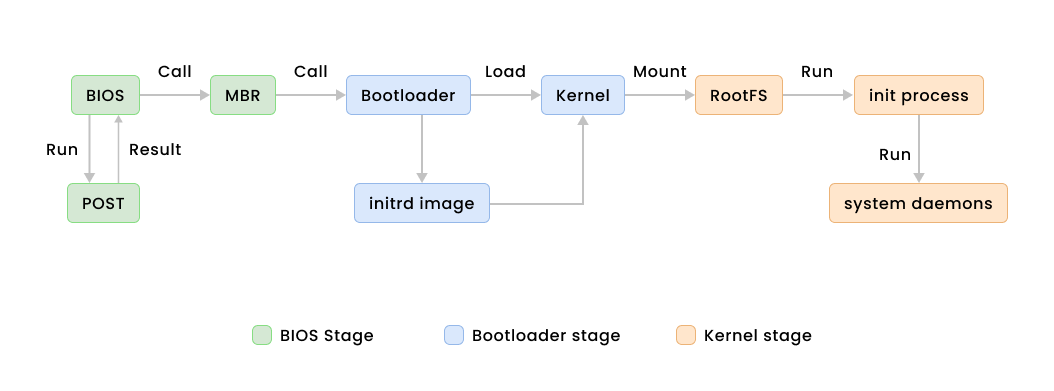
\includegraphics[width=1\textwidth, height=10cm]{images_pfe/bootloader process.png}
  \caption{Processus de démarrage de Kraken OS}
  \label{fig:kbootproc}
\end{figure}

Lors de l’allumage du PC, un signal électrique déclenche le \textbf{POST} (\emph{Power-On Self-Test}), qui initialise le périphérique de démarrage (BIOS ou UEFI).\\

Ensuite, le BIOS/UEFI charge le chargeur d’amorçage (Syslinux) en lisant le fichier de configuration \texttt{isolinux.cfg}, ce qui permet de charger le noyau Linux (\texttt{vmlinuz-kraken}) ainsi que le disque RAM initial (\texttt{initrd}).

Ainsi, pour créer l'ISO, nous devons suivre les étapes suivantes~:
\begin{itemize}
    \item Générer le fichier SquashFS contenant notre système de fichiers
    \item Développer l'image \texttt{initrd}
    \item Configurer le chargeur d'amorçage Syslinux
    \item Développer un script et une application graphique d'installation pour les utilisateurs
    \item Générer le fichier ISO amorçable
\end{itemize}


\section{Générer le fichier SquashFS}

Depuis le chapitre \ref{chap:corebuild}, nous avons construit notre système sur un disque dur, précisément sur un disque VDI de VirtualBox. Ainsi, pour générer l'ISO, nous devons~:
\begin{itemize}
    \item Convertir ce disque VDI en fichier img au format RAW
    \item Monter le fichier (qui contient déjà plusieurs partitions) à l'aide d'outils comme \texttt{kpartx}
    
\end{itemize}

Nous devons ensuite~:
\begin{itemize}
    \item Nettoyer les fichiers de la partition montée (suppression des fichiers temporaires)
    \item Modifier les configurations système (Exemple  le fichier \texttt{/etc/fstab})
    
\end{itemize}

Enfin, nous générons le fichier SquashFS à l'aide de l'outil \texttt{mksquashfs}. Ce fichier contiendra l'intégralité du système dans un format compressé. Nous utilisons l'algorithme de compression \texttt{xz} pour optimiser l'espace.

\begin{figure}[H]
  \centering
  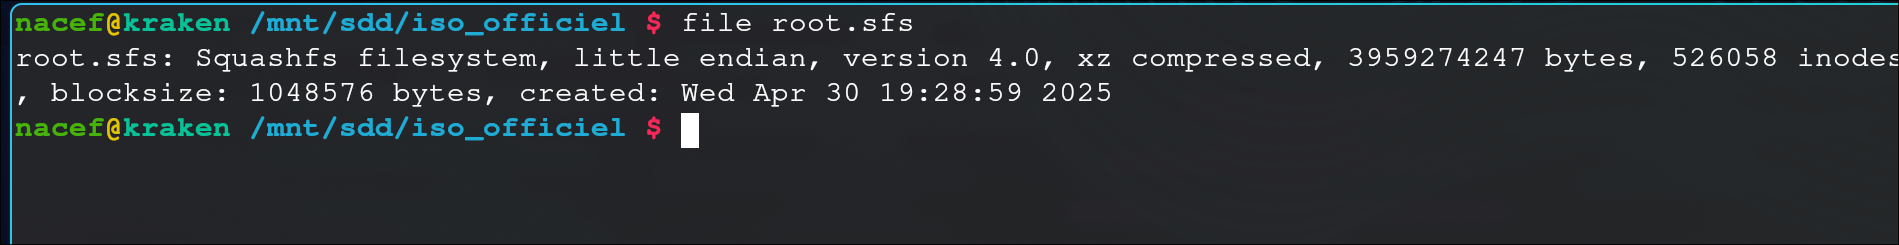
\includegraphics[width=1\textwidth]{images_pfe/rootfsfile.png}
  \caption{Fichier SquashFS généré}
  \label{fig:rootfs}
\end{figure}



\section{Image initrd}

Nous devons maintenant générer l’image \texttt{initrd}.  
Cette image est développée en utilisant \texttt{BusyBox}, une suite logicielle regroupant plusieurs utilitaires Unix dans un seul fichier exécutable.

\noindent
Nous avons besoin que \texttt{BusyBox} prenne en charge les boucles (\texttt{loop}), \texttt{SquashFS} et d’autres fonctionnalités nécessaires.

\begin{figure}[H]
  \centering
  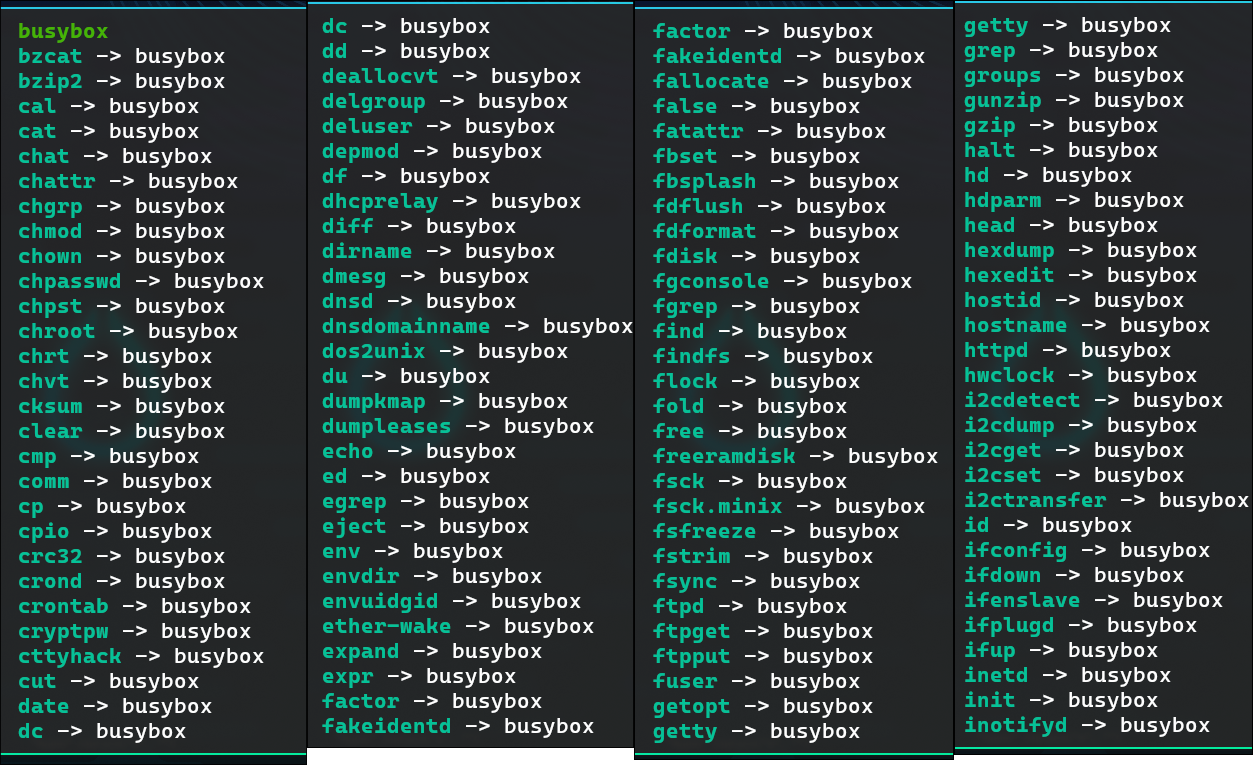
\includegraphics[width=1\textwidth, height=10cm]{images_pfe/busyboxbinary.png}
  \caption{Structure de l'exécutable BusyBox}
  \label{fig:busybox}
\end{figure}

Cet \texttt{initrd} contient un script d’initialisation nommé \texttt{init}, essentiel au montage du fichier \texttt{SquashFS}. Ce script est écrit en \texttt{Bash} et fonctionne exclusivement sur \texttt{Kraken OS}.

\vspace{0.5cm}
\noindent
\textbf{Exemple du contenu du script \texttt{init} :}
\begin{figure}[H]
  \centering
  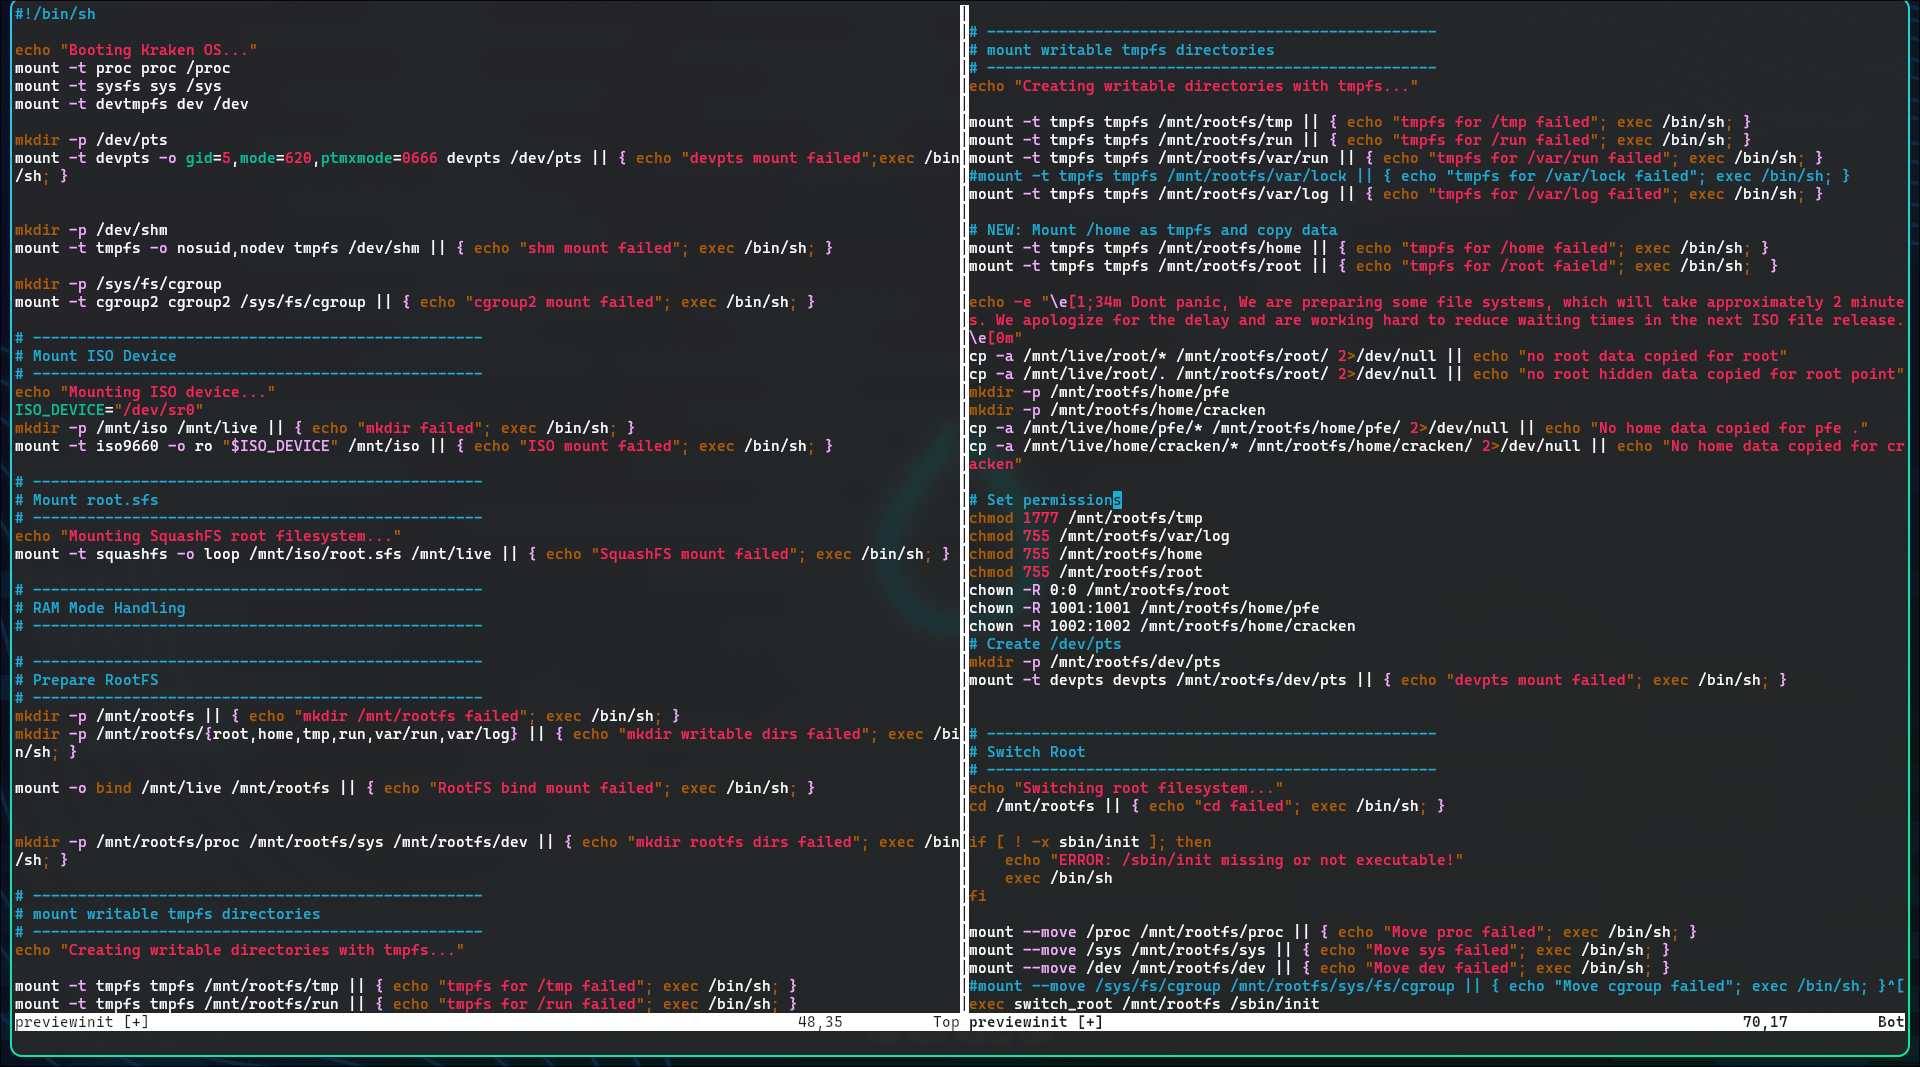
\includegraphics[width=1\textwidth, height=10cm]{images_pfe/intirdinitscript.png}
  \caption{Exemple de script \texttt{init}}
  \label{fig:initscript}
\end{figure}

\vspace{0.3cm}
\noindent
\textbf{Explication :}

L’objectif principal de ce script est de :
\begin{enumerate}
  \item Monter les systèmes de fichiers virtuels (\texttt{proc}, \texttt{dev}, \texttt{sys}, etc.) ;
  \item Monter le contenu du fichier ISO dans \texttt{/mnt/iso}, qui contient notre fichier \texttt{squashfs} ;
  \item Monter le fichier \texttt{squashfs}, contenant notre système de fichiers, dans \texttt{/mnt/live} ;
  \item Copier le contenu de \texttt{squashfs} depuis \texttt{/mnt/live} vers \texttt{/mnt/rootfs} ;
  \item Entrer dans l’environnement \texttt{chroot} situé dans \texttt{/mnt/rootfs} à l’aide de la commande \texttt{switch\_root}.
\end{enumerate}

\vspace{0.5cm}
\noindent
\textbf{Remarque :}

Vous vous demandez peut-être pourquoi nous montons le contenu du fichier \texttt{squashfs} à l’étape 3, puis en copions le contenu à l’étape 4.

C’est parce que la philosophie du système de fichiers \texttt{SquashFS} repose sur le principe du \textbf{mode lecture seule}.  
Pour pouvoir effectuer un \texttt{chroot} dans ce système, il aurait fallu monter le fichier \texttt{squashfs} via un système de fichiers de type \texttt{overlay}.

Cela nécessiterait :
\begin{itemize}
  \item De compiler notre noyau avec le support d’\texttt{overlayfs} ;
  \item De compiler \texttt{BusyBox} avec le support du type \texttt{overlay}.
\end{itemize}

Malheureusement, nous n’avons pas eu le temps de mettre en œuvre cette solution.

Nous avons donc choisi une autre approche :  
Monter le fichier \texttt{squashfs} via un \texttt{bind} dans un répertoire, puis copier son contenu dans un autre répertoire accessible en écriture.  
Ce n’est pas la méthode la plus optimale, mais elle est fonctionnelle pour cette version.  
Nous prévoyons d’améliorer cette partie dans une prochaine version de l’image ISO.

\vspace{0.5cm}
\noindent
Après cela, nous générons le fichier \texttt{initrd} à l’aide des outils \texttt{find}, \texttt{cpio}, \texttt{gzip}, etc.

\begin{figure}[H]
  \centering
  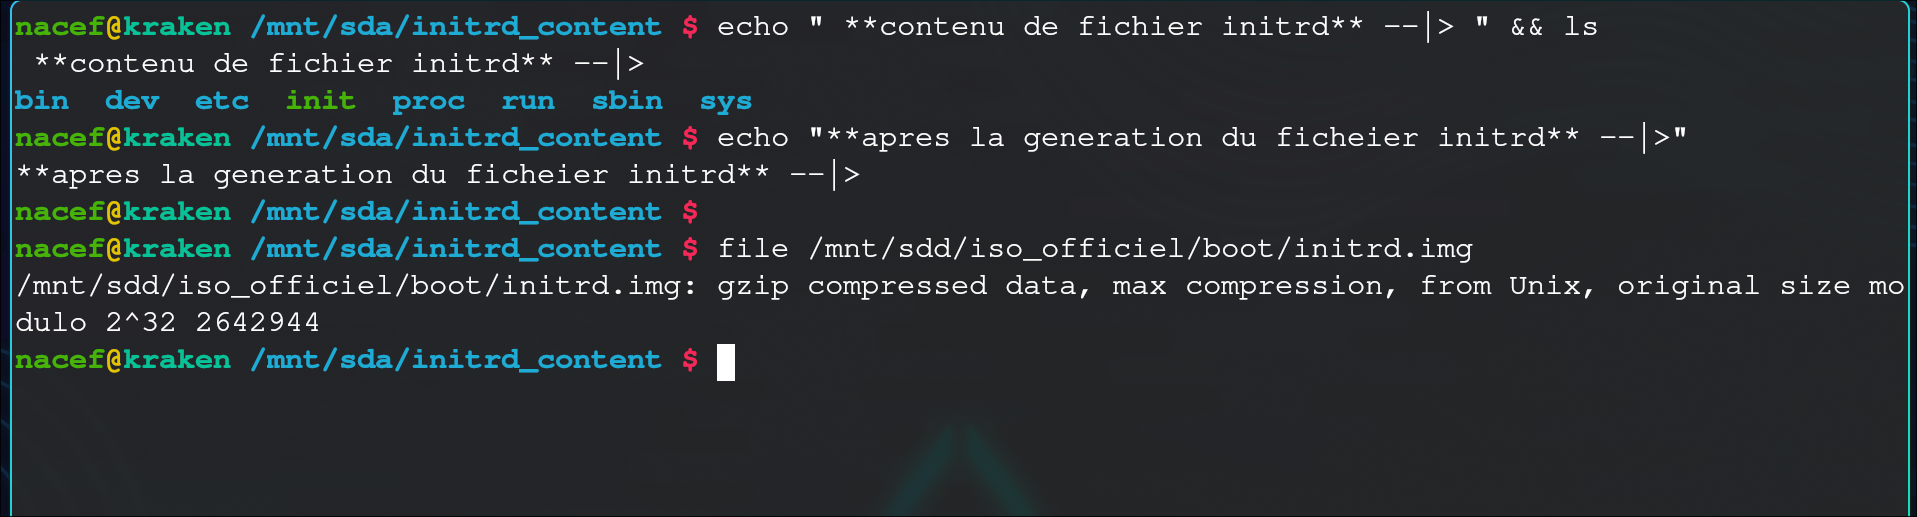
\includegraphics[width=1\textwidth, height=10cm]{images_pfe/initrdcontentfile.png}
  \caption{Contenu du fichier \texttt{initrd}}
  \label{fig:initcontent}
\end{figure}

\noindent
\textcolor{blue}{Le code source du fichier \texttt{initrd} et du script \texttt{init} est disponible dans \cite{initrd}.}


\section{Bootloader Syslinux}

Dans l'environnement ISO, il est recommandé d'utiliser le chargeur de démarrage Syslinux au lieu de GRUB pour des raisons de simplicité. Ensuite, pendant l'installation du système depuis l'environnement live vers le disque désiré, nous utiliserons le chargeur de démarrage GRUB. 

Il y a une configuration critique à effectuer dans Syslinux pour garantir un démarrage correct.\\
Exemple du fichier \texttt{isolinux.cfg} :

\begin{figure}[H]
  \centering
  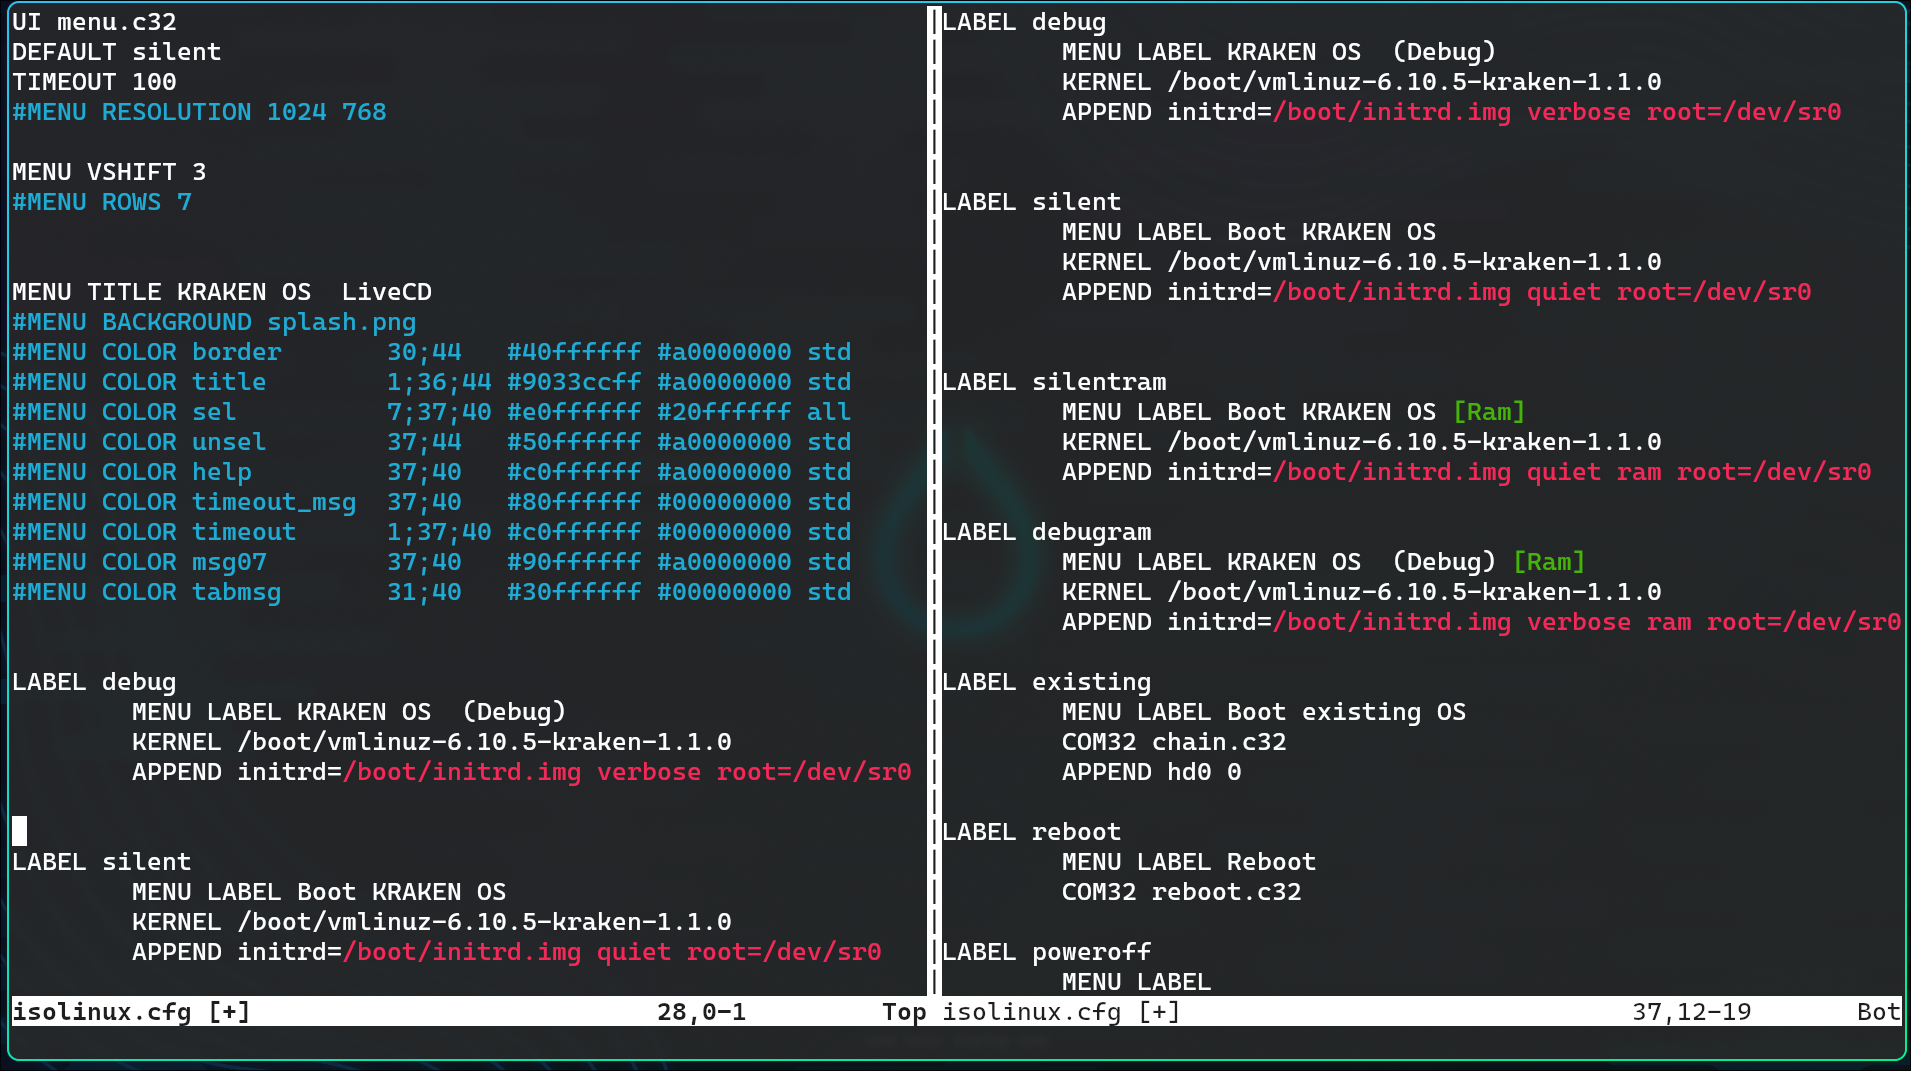
\includegraphics[width=1\textwidth, height=10cm]{images_pfe/cfgisolinuxcorrect.png}
  \caption{Exemple fichier isolinux.cfg }
  \label{fig:isolinux}
\end{figure}

Exemple de menu de syslinux bootloader :

\begin{figure}[H]
  \centering
  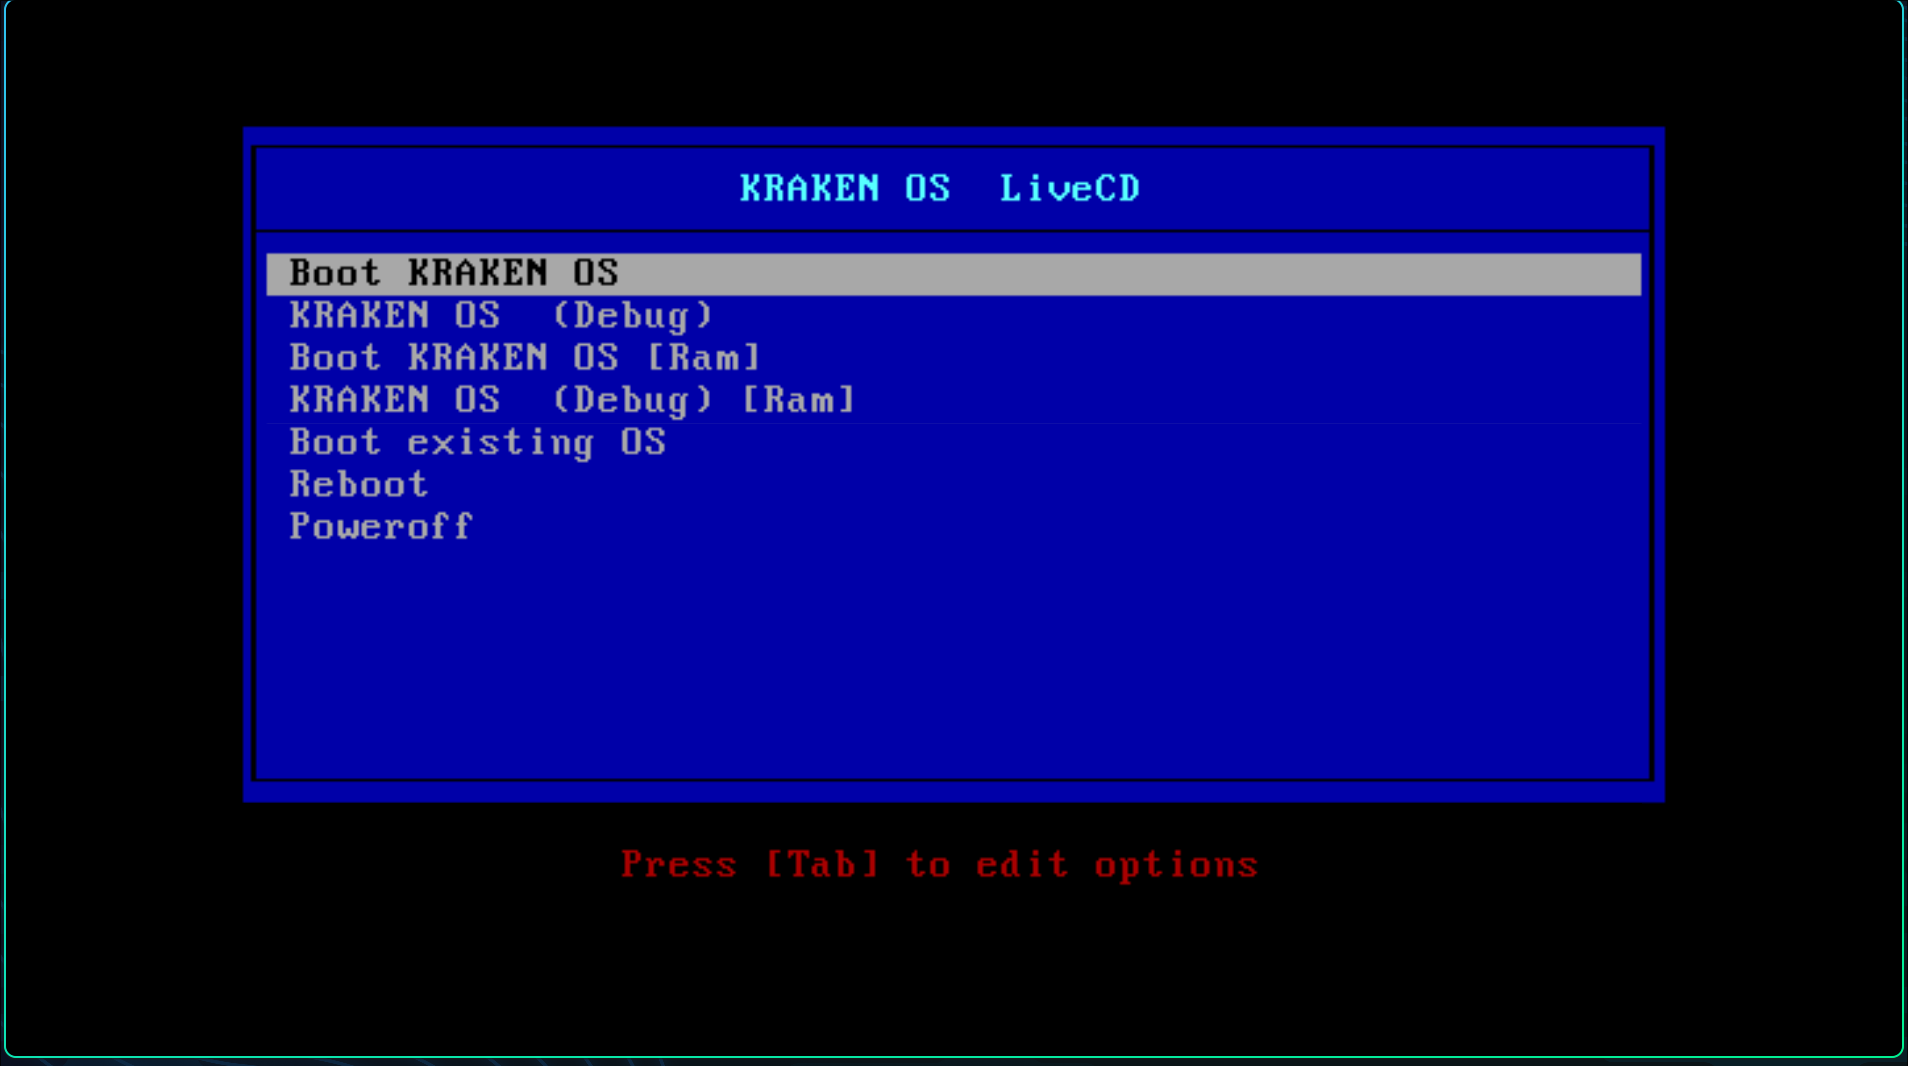
\includegraphics[width=1\textwidth, height=10cm]{images_pfe/syslinuxmenu.png}
  \caption{Menu de démarrage Syslinux}
  \label{fig:syslinux}
\end{figure}
\textcolor{blue}{Pour en savoir plus sur syslinux, référez-vous à \cite{syslinux}.}\\
\section{Script d'installation }
\label{secc:sctipttui}

Après avoir démarré l'ISO , nous devons fournir à l'utilisateur un script capable d'installer l'ISO depuis \textbf{l'environnement live} vers le \textbf{disque dur local}.

Ce script gère plusieurs aspects, tels que la partition du disque, le montage du disque, la copie des fichiers système, la configuration du chargeur de démarrage dans le nouveau système, la création d'un utilisateur, la configuration de la langue, de la disposition du clavier, la configuration de l'environnement du nouvel utilisateur, l'édition du fichier \texttt{/etc/fstab}, l'activation de thèmes pour GRUB, SDDM, etc.

Ce script est développé spécialement pour Kraken OS ; si vous tentez de l'exécuter sur une autre machine ou distribution, il échouera.




\textbf{Commande :}

\begin{lstlisting}
./kraken_install.sh "disk_name" "home_on" "swap_on" "username" "userpass" 
  "system_language" "keyboard_layout" "hostname" "time_zone"
\end{lstlisting}

\textbf{Exemple d'utilisation :}
\begin{lstlisting}
sudo ./kraken_install.sh /dev/sda yes yes n1cef password en_US.UTF-8 us kraken /Africa/Tunis
\end{lstlisting}



\textbf{Exemple de parametre valide }
\begin{table}[H]
    \centering
    \small
    \begin{tabularx}{\textwidth}{|c|c|X|}
        \hline
        \textbf{Paramètre} & \textbf{Exemples} & \textbf{Description} \\
        \hline
        \texttt{disk-name} & \texttt{/dev/sda}, \texttt{/dev/sdb} & Chemin complet vers le disque cible \\
        \hline
        \texttt{home-on} & \texttt{yes}, \texttt{no} & Créer une partition séparée pour \texttt{/home} \\
        \hline
        \texttt{swap-on} & \texttt{yes}, \texttt{no} & Créer une partition de swap \\
        \hline
        \texttt{username} & \texttt{n1cef} & Nom du compte utilisateur principal  \\
        \hline
        \texttt{userpass} & \texttt{"MotDePasse123!"} & Mot de passe de l'utilisateur principal  \\
        \hline
        \texttt{system-language} & \texttt{fr-FR.UTF-8}, \texttt{en-US.UTF-8}, \texttt{ar-SA.UTF-8} & Langue et paramètre régional du système \\
        \hline
        \texttt{keyboard-layout} & \texttt{fr}, \texttt{us}, \texttt{ar} & Code de disposition du clavier (Français, Anglais, Arabe) \\
        \hline
        \texttt{hostname} & \texttt{kraken} & Nom d'hôte du système  \\
        \hline
        \texttt{time-zone} & \texttt{/Europe/Paris}, \texttt{/Africa/Tunis}, \texttt{/Asia/Dubai} & Fuseau horaire au format \texttt{/Région/Ville} \\
        \hline
    \end{tabularx}
    \caption{Paramètres de configuration système}
    \label{tab:system-config-params}
\end{table}


%\begin{figure}[H]
 % \centering
 % 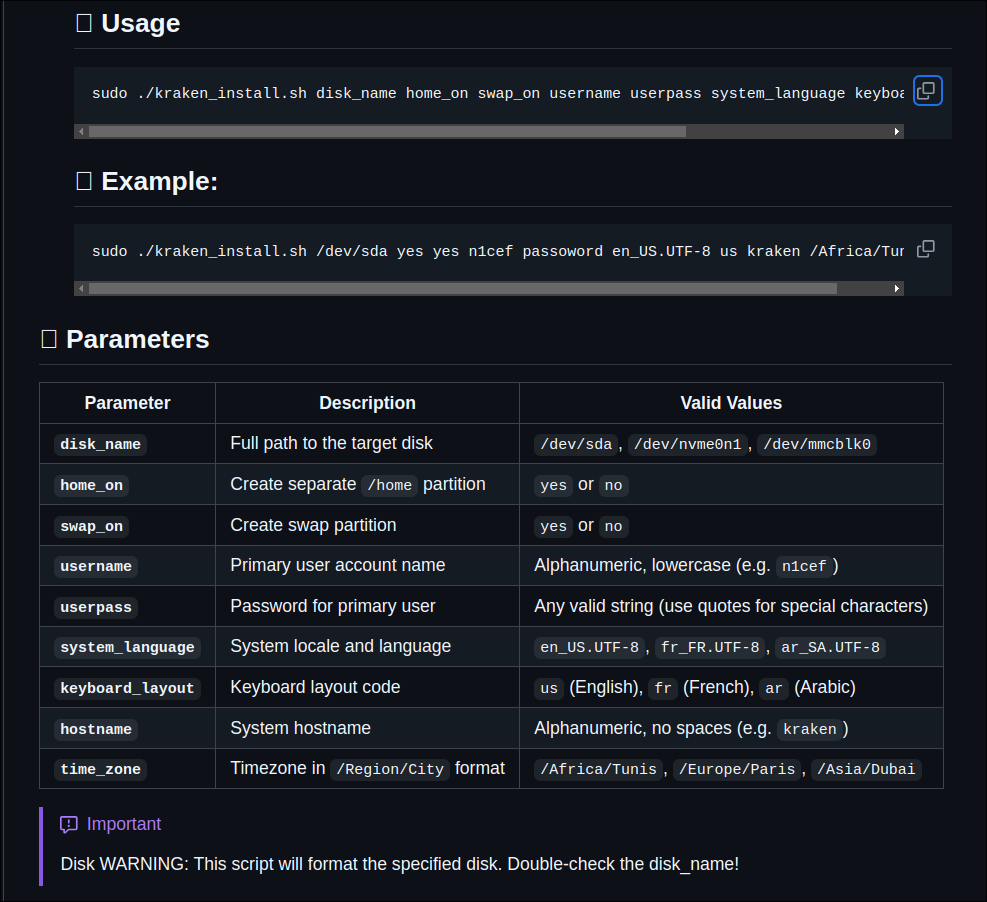
\includegraphics[width=1\textwidth, height=14cm]{images_pfe/diskuses.png}
 % \caption{ exemple d utilisation de script d’installation }
 % \label{fig:diskuses}
%\end{figure}



\textcolor{blue}{Le code source du script d’installation est disponible dans  \cite{installateur_tui}.}


\section{Application graphique "Kraken Installer" }
\label{secc:graphapp}


Le script d'installation Kraken créé précédemment peut être difficile à utiliser pour un utilisateur Linux non expert. Ainsi, nous avons choisi de développer une application graphique pour rendre le processus d'installation du système plus convivial.




Cette application fournit simplement à l'utilisateur des champs et des options pour sélectionner la langue du système, configurer son nom d'utilisateur et son mot de passe, choisir la disposition du clavier, sélectionner le disque et la partition, choisir les paquets à installer dans le nouveau système, etc.

\textbf{Fonctionnalité clé} : Génération d'un fichier JSON stockant toutes ces configurations pour l'installation ultérieure du système.


\begin{figure}[H]
  \centering
  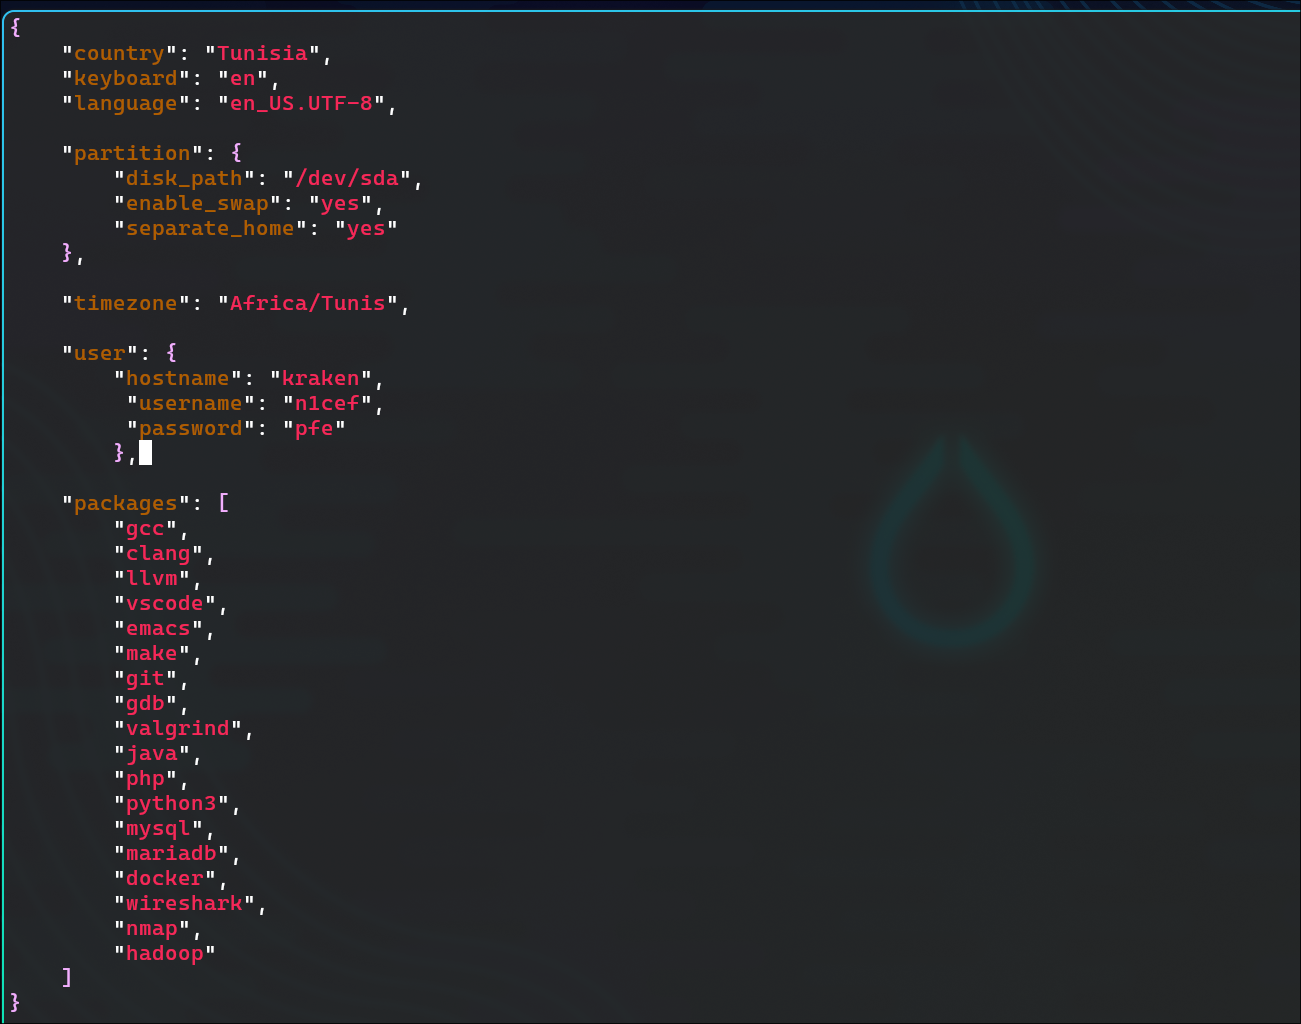
\includegraphics[width=1\textwidth, height=10cm]{images_pfe/jsonsettings.png}
  \caption{Exemple de fichier settings.json généré}
  \label{fig:jsonsettings}
\end{figure}


\clearpage
\subsection*{Langages et frameworks utilisés}
\begin{figure}[hbt!]
  \centering
  \begin{minipage}[b]{0.18\textwidth}
    
\includegraphics[width=\textwidth]{images_pfe/c+++.png}
    \caption{C++17/20}
  \end{minipage}\hfill
  \begin{minipage}[b]{0.18\textwidth}
    
\includegraphics[width=\textwidth]{images_pfe/xml.png}
    \caption{Qt XML}
  \end{minipage}\hfill
  \begin{minipage}[b]{0.18\textwidth}
    
\includegraphics[width=\textwidth]{images_pfe/qt6.jpeg}
    \caption{Qt6 Framework}
  \end{minipage}\hfill
  \begin{minipage}[b]{0.18\textwidth}
    
\includegraphics[width=\textwidth]{images_pfe/css.jpeg}
    \caption{Qt CSS}
  \end{minipage}\hfill
  \caption{Stack technique de l'installateur graphique}
  \label{fig:krakenistallerlanguage}
\end{figure}
\FloatBarrier
 
  
  
  
 


\subsection{ Les pages de l'application}


\subsection{ Page principale}
\begin{figure}[H]
  \centering
  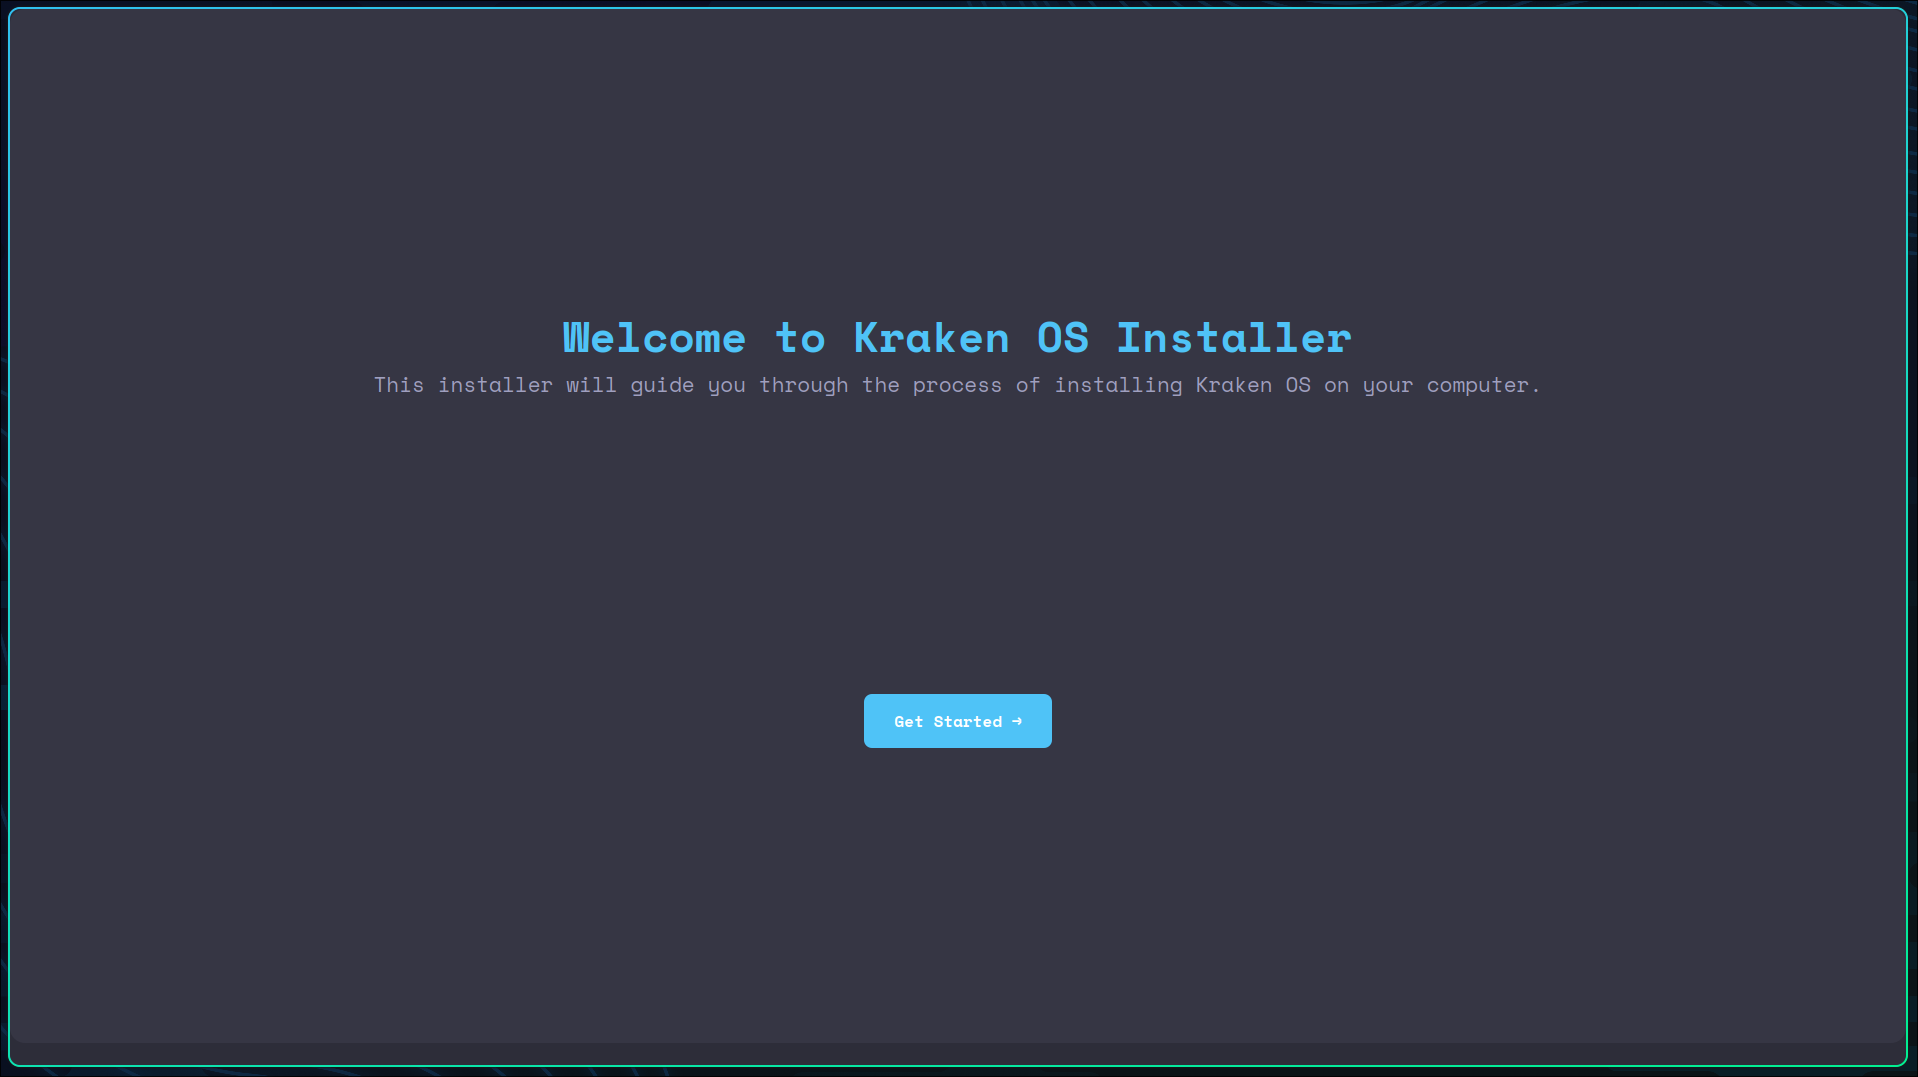
\includegraphics[width=1\textwidth, height=10cm]{images_pfe/mainwindow.png}
  \caption{Page principale de l'application Kraken Installer (page d'accueil)}
  \label{fig:mwindow}
\end{figure}



%\subsection{ Page de bienvenue}

%\begin{figure}[H]
 % \centering
 % 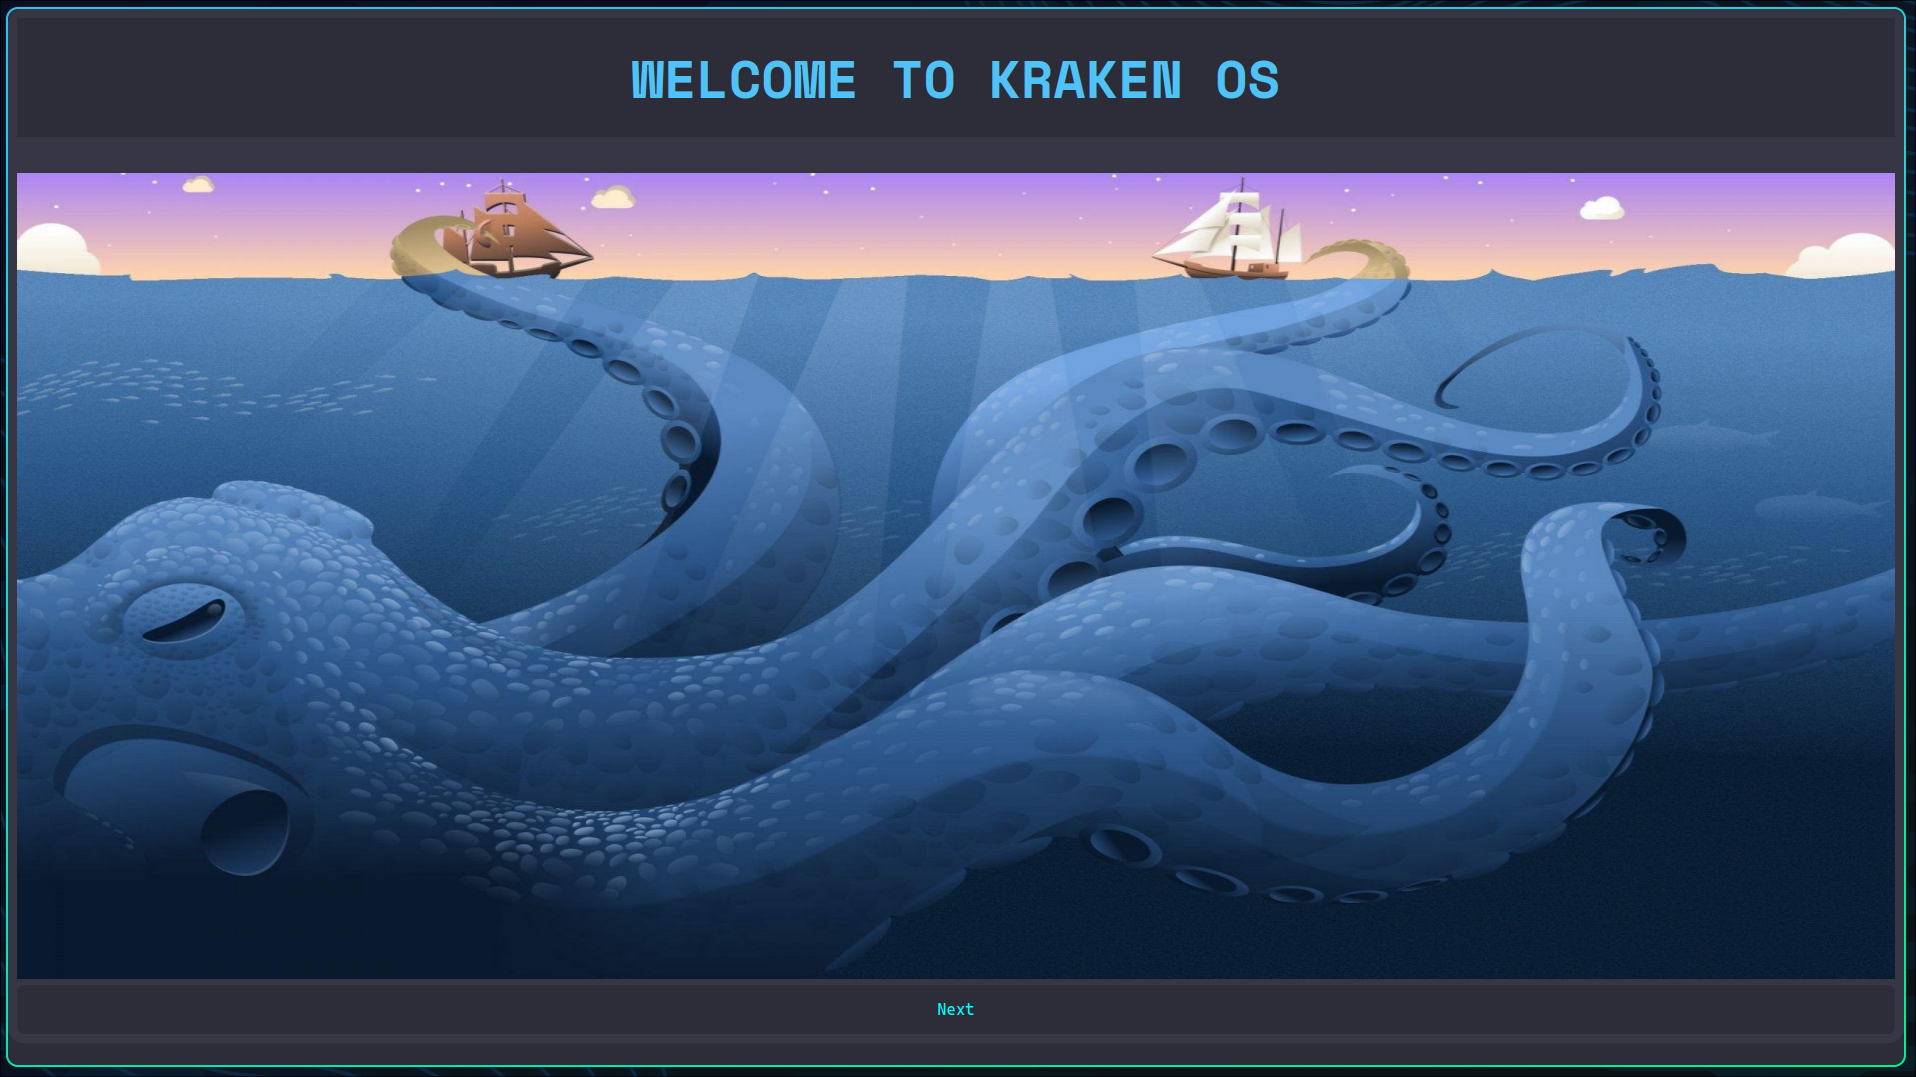
\includegraphics[width=1\textwidth, height=10cm]{images_pfe/welcome.png}
 % \caption{Page de bienvenue de l'application Kraken Installer}
 % \label{fig:wlecompage}
%\end{figure}




\subsection{Page de configuration du clavier}
\begin{figure}[H]
  \centering
  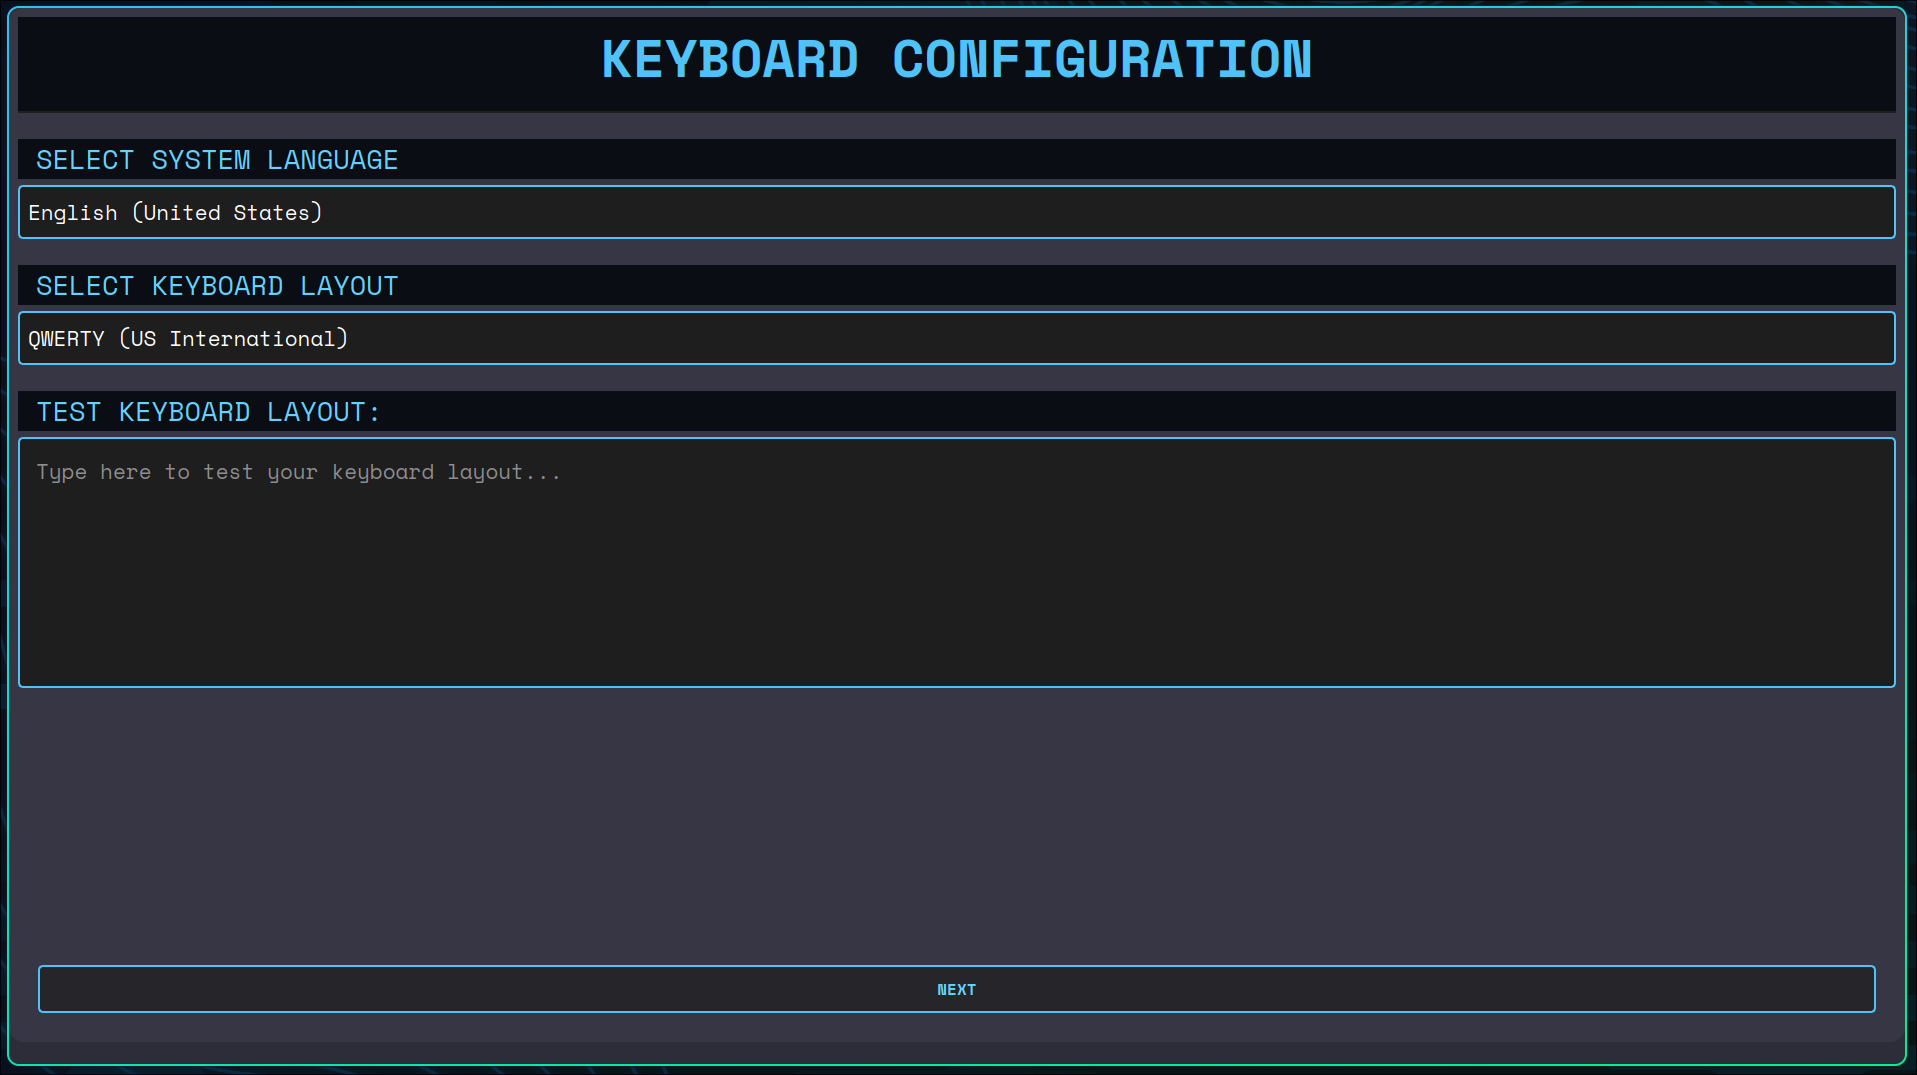
\includegraphics[width=1\textwidth, height=10cm]{images_pfe/keyboard.png}
  \caption{Interface de configuration clavier de l'application \textsc{Kraken Installer}}
  \label{fig:keyboardpage}
\end{figure}

\textbf{Fonctionnalité} : Cette page propose à l'utilisateur :
\begin{itemize}
    \item Deux menus déroulants (\texttt{QComboBox}) pour :
    \begin{itemize}
        \item Sélectionner la langue du système
        \item Choisir la disposition du clavier
    \end{itemize}
    \item Un bouton de validation qui :
    \begin{itemize}
        \item Sauvegarde les paramètres dans un fichier \texttt{JSON}
        \item Redirige vers la page suivante
    \end{itemize}
\end{itemize}



\subsection{ Page de configuration de la localisation}

\begin{figure}[H]
  \centering
  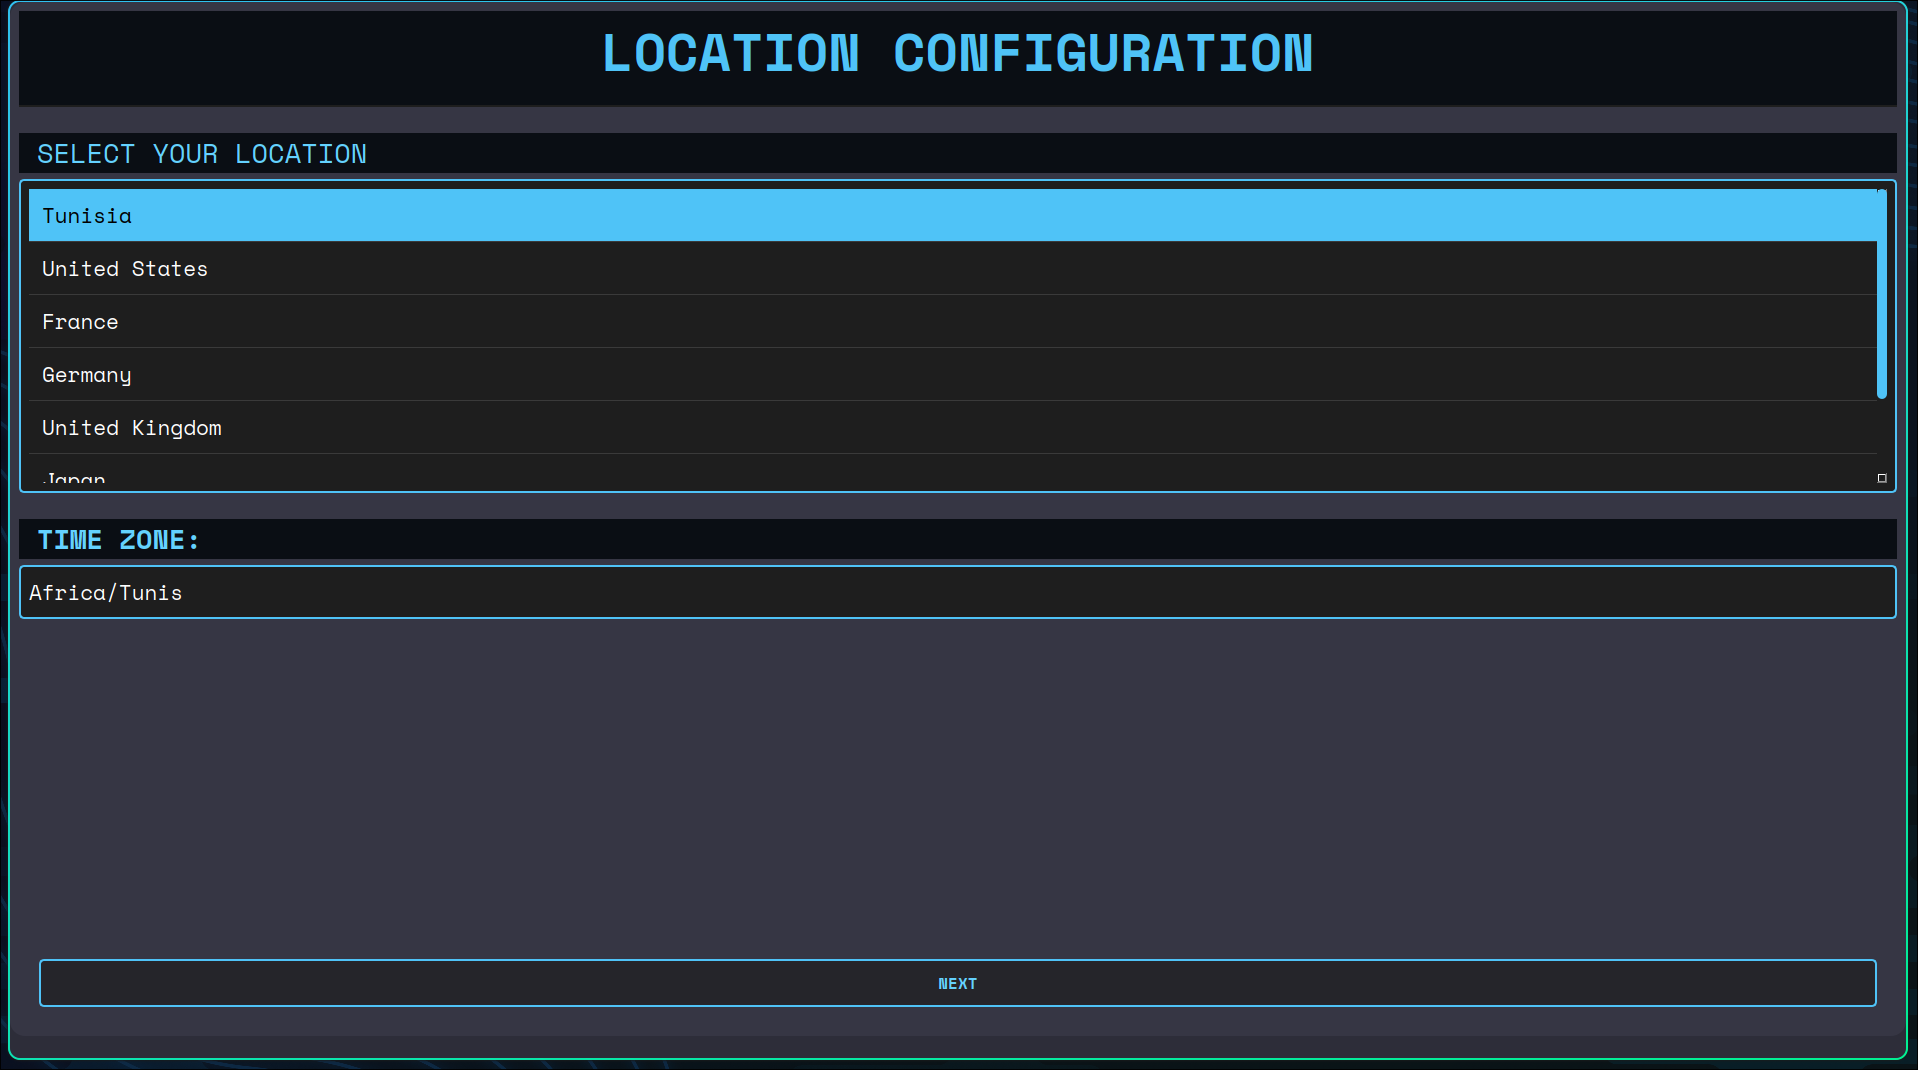
\includegraphics[width=1\textwidth, height=10cm]{images_pfe/location.png}
  \caption{Interface de configuration géographique de l'application \textsc{Kraken Installer}}
  \label{fig:locationpage}
\end{figure}

\textbf{Fonctionnalité} : Cette page permet à l'utilisateur de :
\begin{itemize}
    \item Sélectionner sa région géographique via un \texttt{QListWidget}
    \item Choisir son fuseau horaire (ex: \texttt{Africa/Tunis}) via un \texttt{QComboBox}
    \item Valider ces paramètres avec un bouton \textit{Suivant} qui :
    \begin{itemize}
        \item Sauvegarde les configurations dans le fichier \texttt{JSON}
        \item Redirige vers l'étape suivante de l'installation
    \end{itemize}
\end{itemize}



\subsection{Page de configuration de l'utilisateur}

\begin{figure}[H]
  \centering
  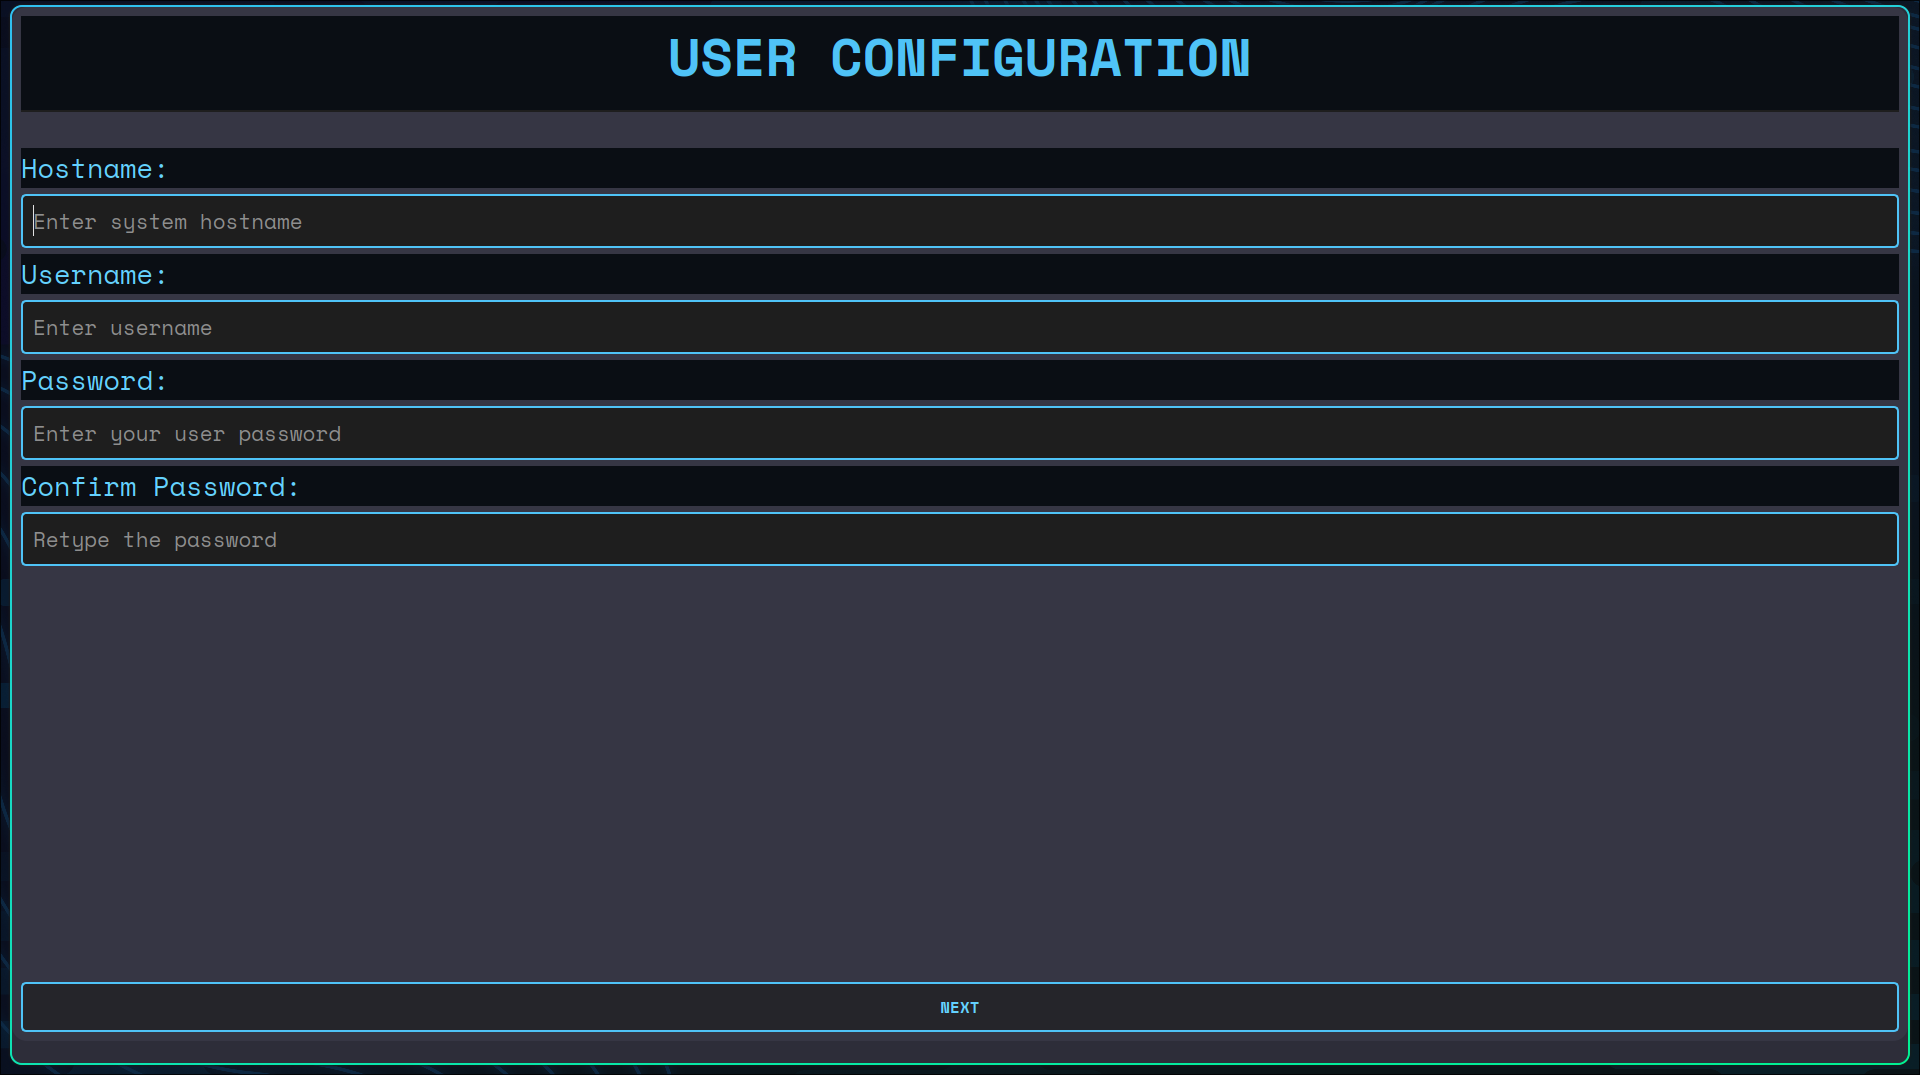
\includegraphics[width=1\textwidth, height=10cm]{images_pfe/user.png}
  \caption{Interface de configuration utilisateur de l'application \textsc{Kraken Installer}}
  \label{fig:userpage}
\end{figure}


\textbf{Fonctionnalité} : Cette interface permet à l'utilisateur de :
\begin{itemize}
    \item Définir le nom d'hôte du système via un \texttt{QLineEdit}
    \item Créer un compte utilisateur avec :
    \begin{itemize}
        \item Un champ \texttt{QLineEdit} pour le nom d'utilisateur
        \item Deux champs de mot de passe (saisie + confirmation)
    \end{itemize}
    \item Valider via un bouton \textit{Suivant} qui :
    \begin{itemize}
        \item Vérifie la concordance des mots de passe
        \item Signale les champs incomplets
        \item Sauvegarde les paramètres dans le fichier \texttt{JSON}
        \item Redirige vers l'étape suivante
    \end{itemize}
\end{itemize}

\textbf{Note de sécurité} : 
\begin{itemize}
    \item Les mots de passe doivent être identiques
    \item Tous les champs sont obligatoires
    \item En cas d'erreur, l'application bloque la progression et demande une correction
\end{itemize}



\subsection{Page de partitionnement du disque}

\begin{figure}[H]
  \centering
  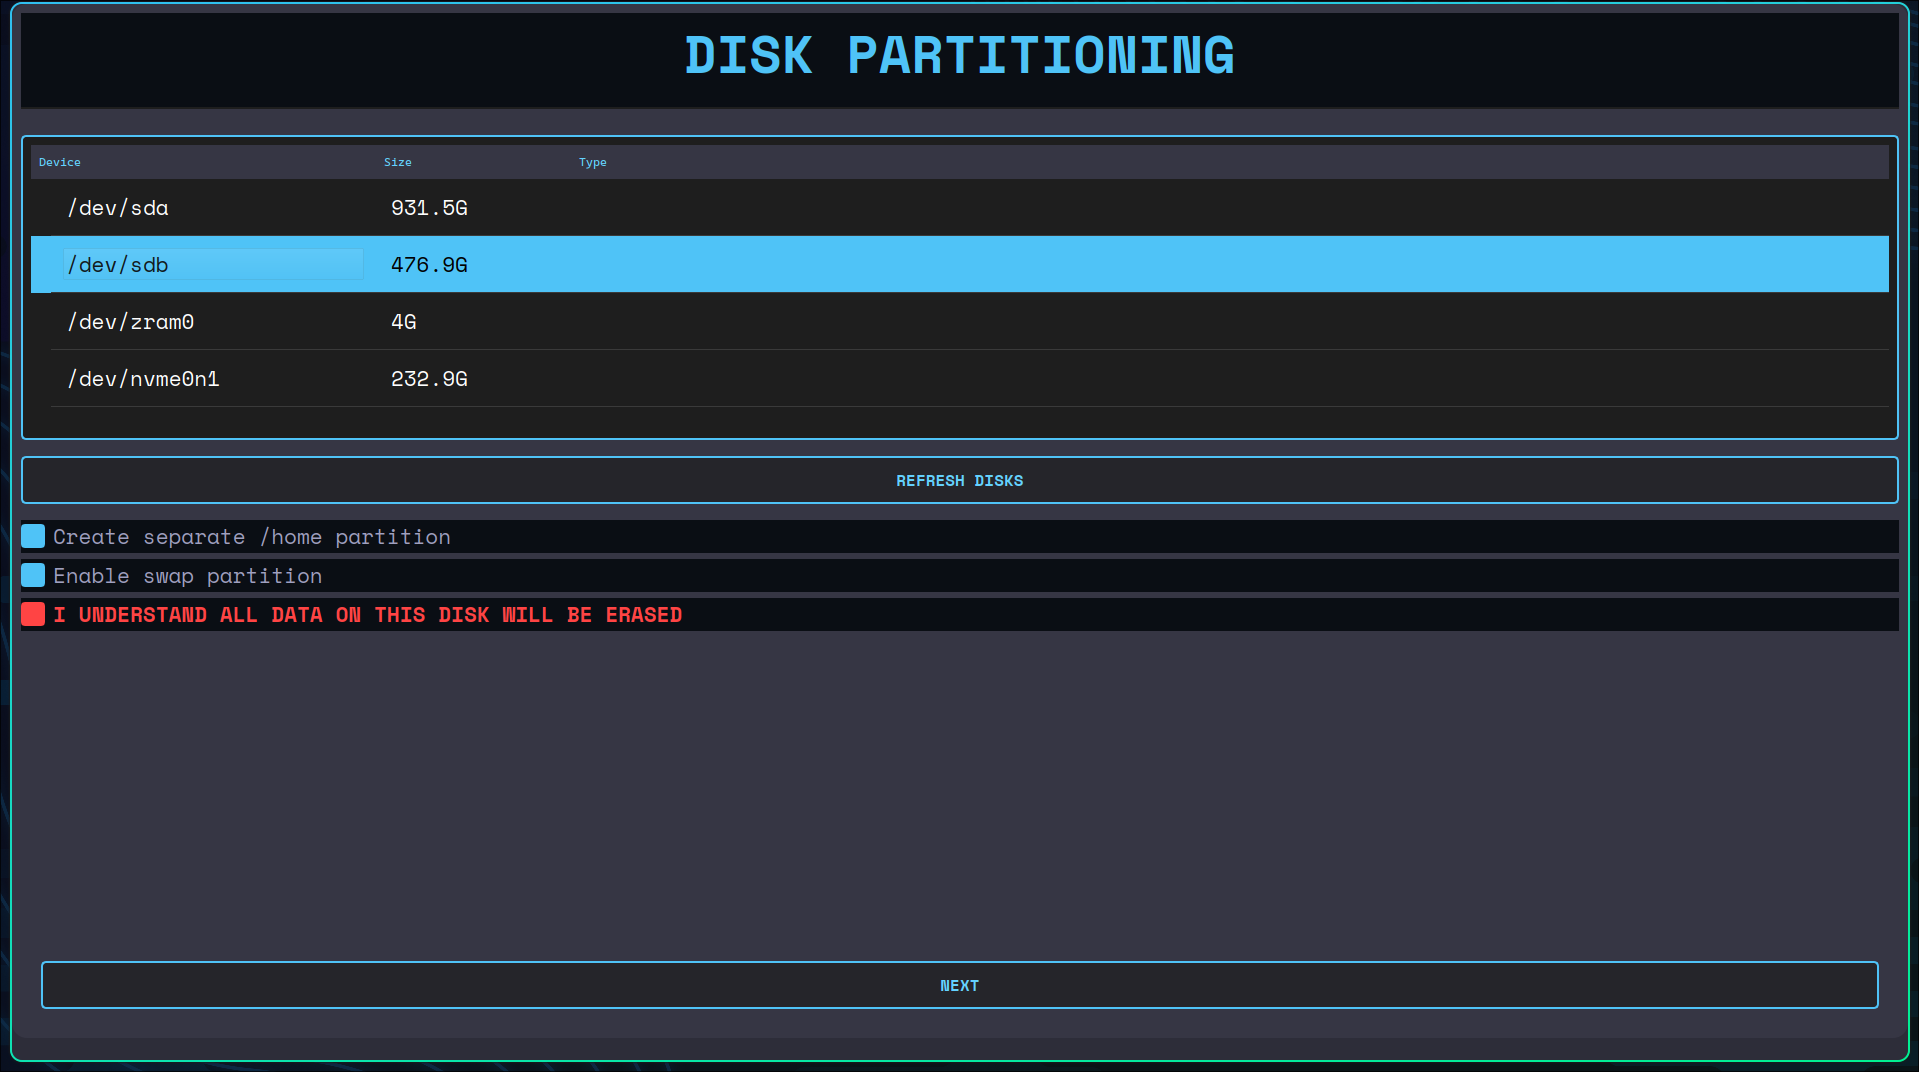
\includegraphics[width=1\textwidth, height=10cm]{images_pfe/disk.png}
  \caption{Interface de partitionnement de disque de l'application \textsc{Kraken Installer}}
  \label{fig:diskpage}
\end{figure}

\label{subsec:disk-partitioning}

\textbf{Fonctionnalités} :
\begin{itemize}
    \item \texttt{QTreeWidget} détectant automatiquement les disques disponibles
    \item Bouton \textit{Actualiser les disques} (\texttt{QPushButton}) pour mettre à jour la liste des disques 
    \item Options de partitionnement via des cases à cocher (\texttt{QCheckBox}) :
    \begin{itemize}
        \item Créer une partition \texttt{/home} séparée
        \item Activer une partition \texttt{swap}
        \item Case obligatoire :  Je confirme avoir compris que toutes les données du disque seront effacées
    \end{itemize}
    \item Validation via bouton \textit{Suivant} qui :
    \begin{itemize}
        \item Vérifie la sélection de la case de confirmation
        \item Sauvegarde la configuration dans le fichier \texttt{JSON}
        \item Redirige vers l'étape suivante
    \end{itemize}
\end{itemize}

\


\subsection{Page de sélection des paquets}



\label{subsec:package-selection}
\begin{figure}[H]
  \centering
  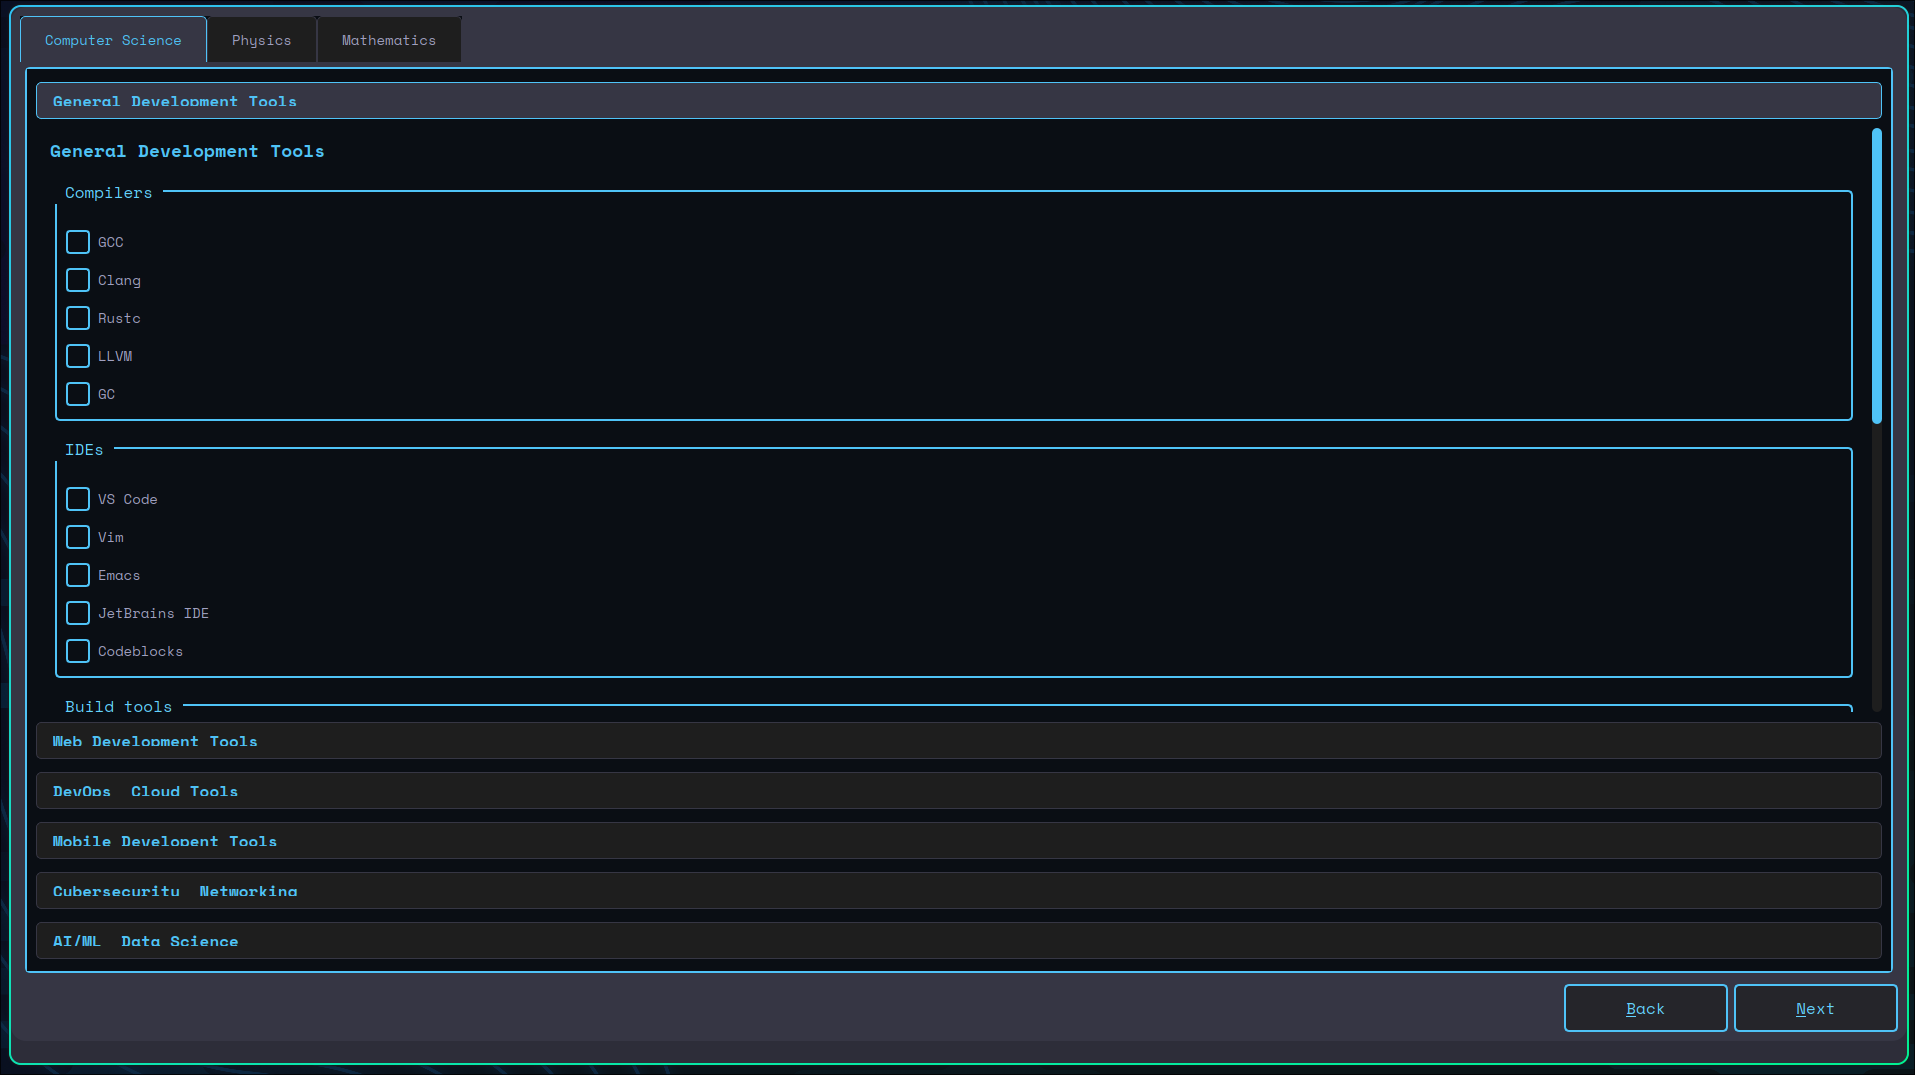
\includegraphics[width=1\textwidth, height=10cm]{images_pfe/packages.png}
  \caption{Interface de sélection des paquets de l'application \textsc{Kraken Installer}}
  \label{fig:packagepage}
\end{figure}



\textbf{Fonctionnalités} :  
Cette interface propose à l'utilisateur :
\begin{itemize}
    \item 3 onglets thématiques via \texttt{QTabWidget} :
    \begin{itemize}
        \item Informatique
        \item Mathématiques
        \item Physique
    \end{itemize}
    
    \item Sous-catégories détaillées (exemple pour l'onglet \textit{Informatique}) :
    \begin{itemize}
        \item Outils de développement général
        \item Outils web
        \item DevOps \& Cloud
        \item Développement mobile
        \item Cybersécurité
        \item IA/ML (Intelligence Artificielle et Machine Learning)
    \end{itemize}
    
    \item Sélection via \texttt{QCheckBox} pour chaque paquet
    \item Validation via \texttt{QPushButton} qui :
    \begin{itemize}
        \item Sauvegarde les sélections dans un tableau JSON
        \item Redirige vers l'étape suivante
    \end{itemize}
\end{itemize}





\subsection{Page de progression de l'installation}
\label{subsec:installation-progress}

\begin{figure}[H]
  \centering
  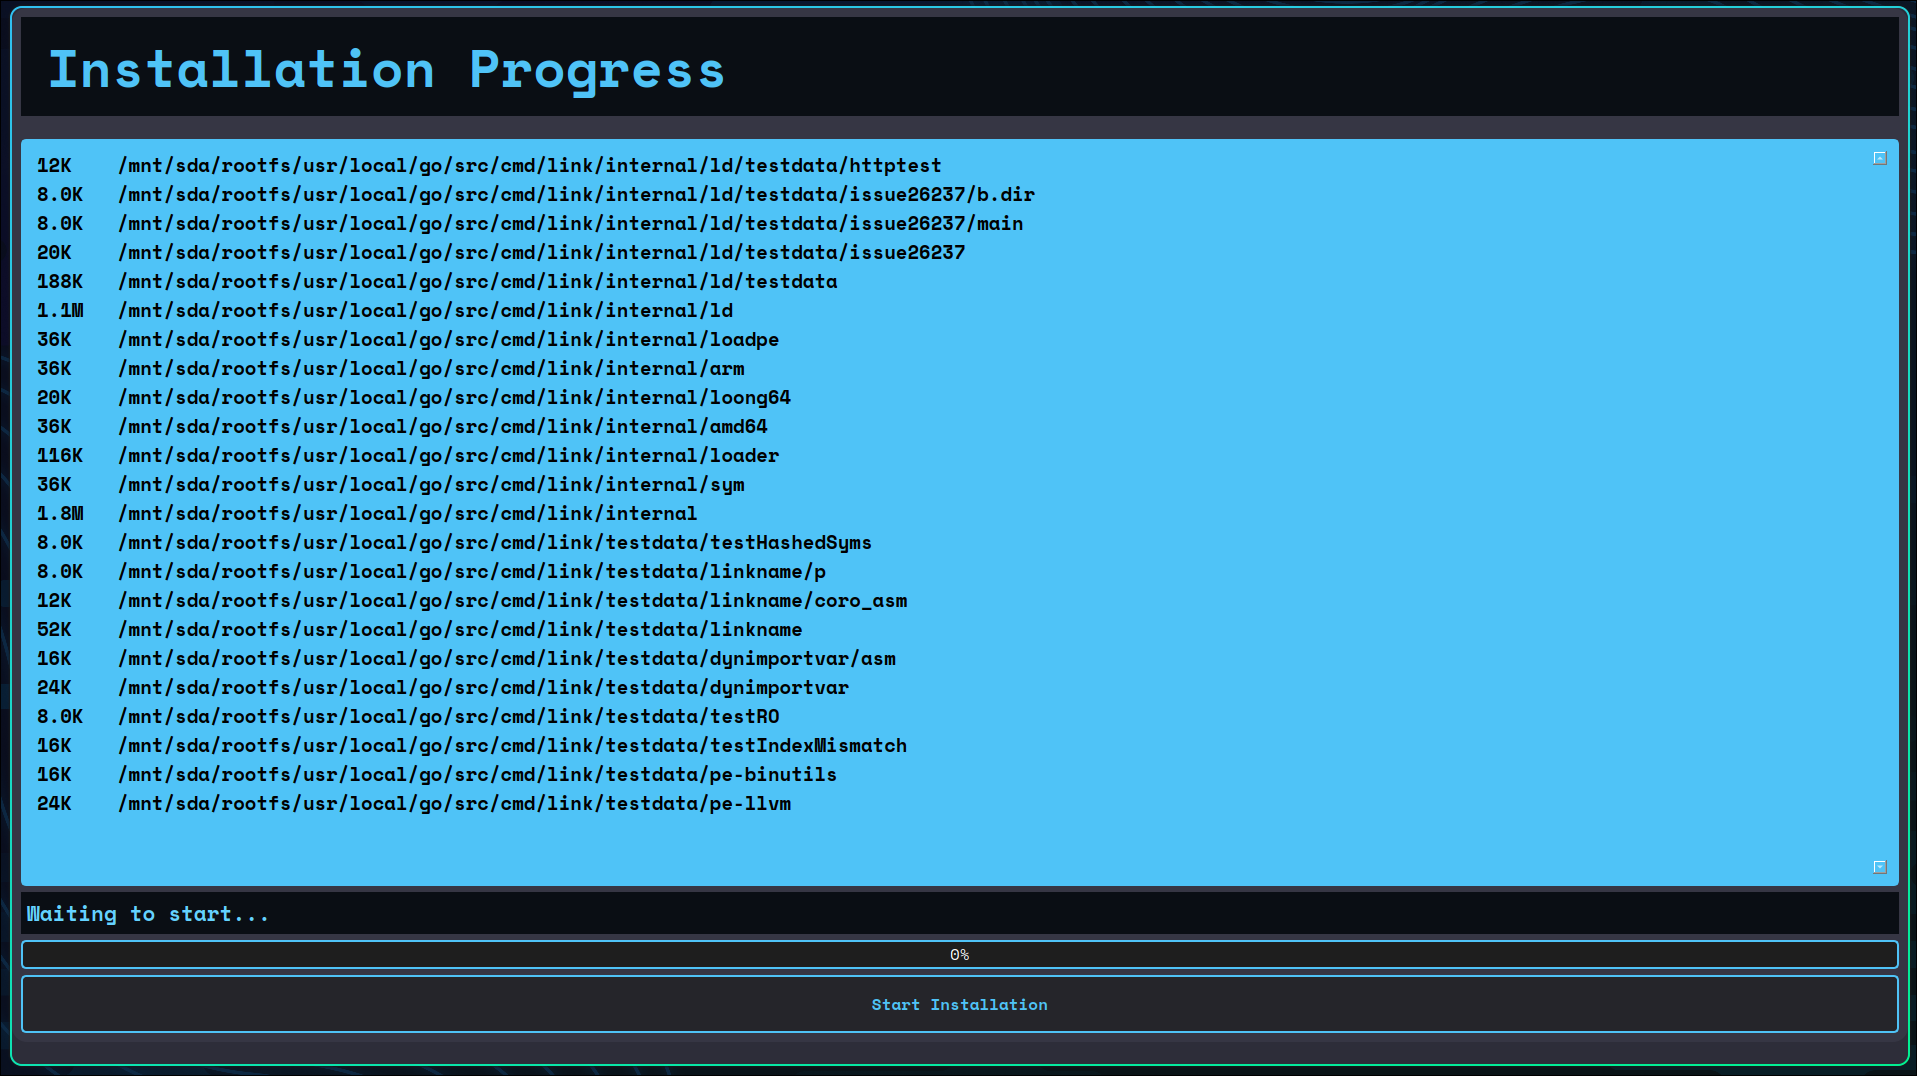
\includegraphics[width=1\textwidth, height=10cm]{images_pfe/installation.png}
  \caption{Interface de progression de l'installation dans \textsc{Kraken Installer}}
  \label{fig:install-page}
\end{figure}

\textbf{Fonctionnalités} :
\begin{itemize}
    \item Bouton \textit{Démarrer l'installation} (\texttt{QPushButton}) lançant le processus :
    \begin{itemize}
        \item Extraction des paramètres  depuis le fichier \texttt{JSON}
        \item Exécution d'un script dinstallation  \textcolor{blue}{\ref{secc:sctipttui}}   avec les paramètres en entrée
    \end{itemize}
    
    \item Widget \texttt{QPlainTextEdit} affichant :
    \begin{itemize}
        \item Les logs d'installation en temps réel
        \item La progression des étapes (partitionnement, copie des fichiers, configuration...)
        
    \end{itemize}
    
    \item Gestion visuelle de la progression :
    \begin{itemize}
        \item Barre de progression intégrée 
       
    \end{itemize}
\end{itemize}




\subsection{Page de redémarrage}


\begin{figure}[H]
  \centering
  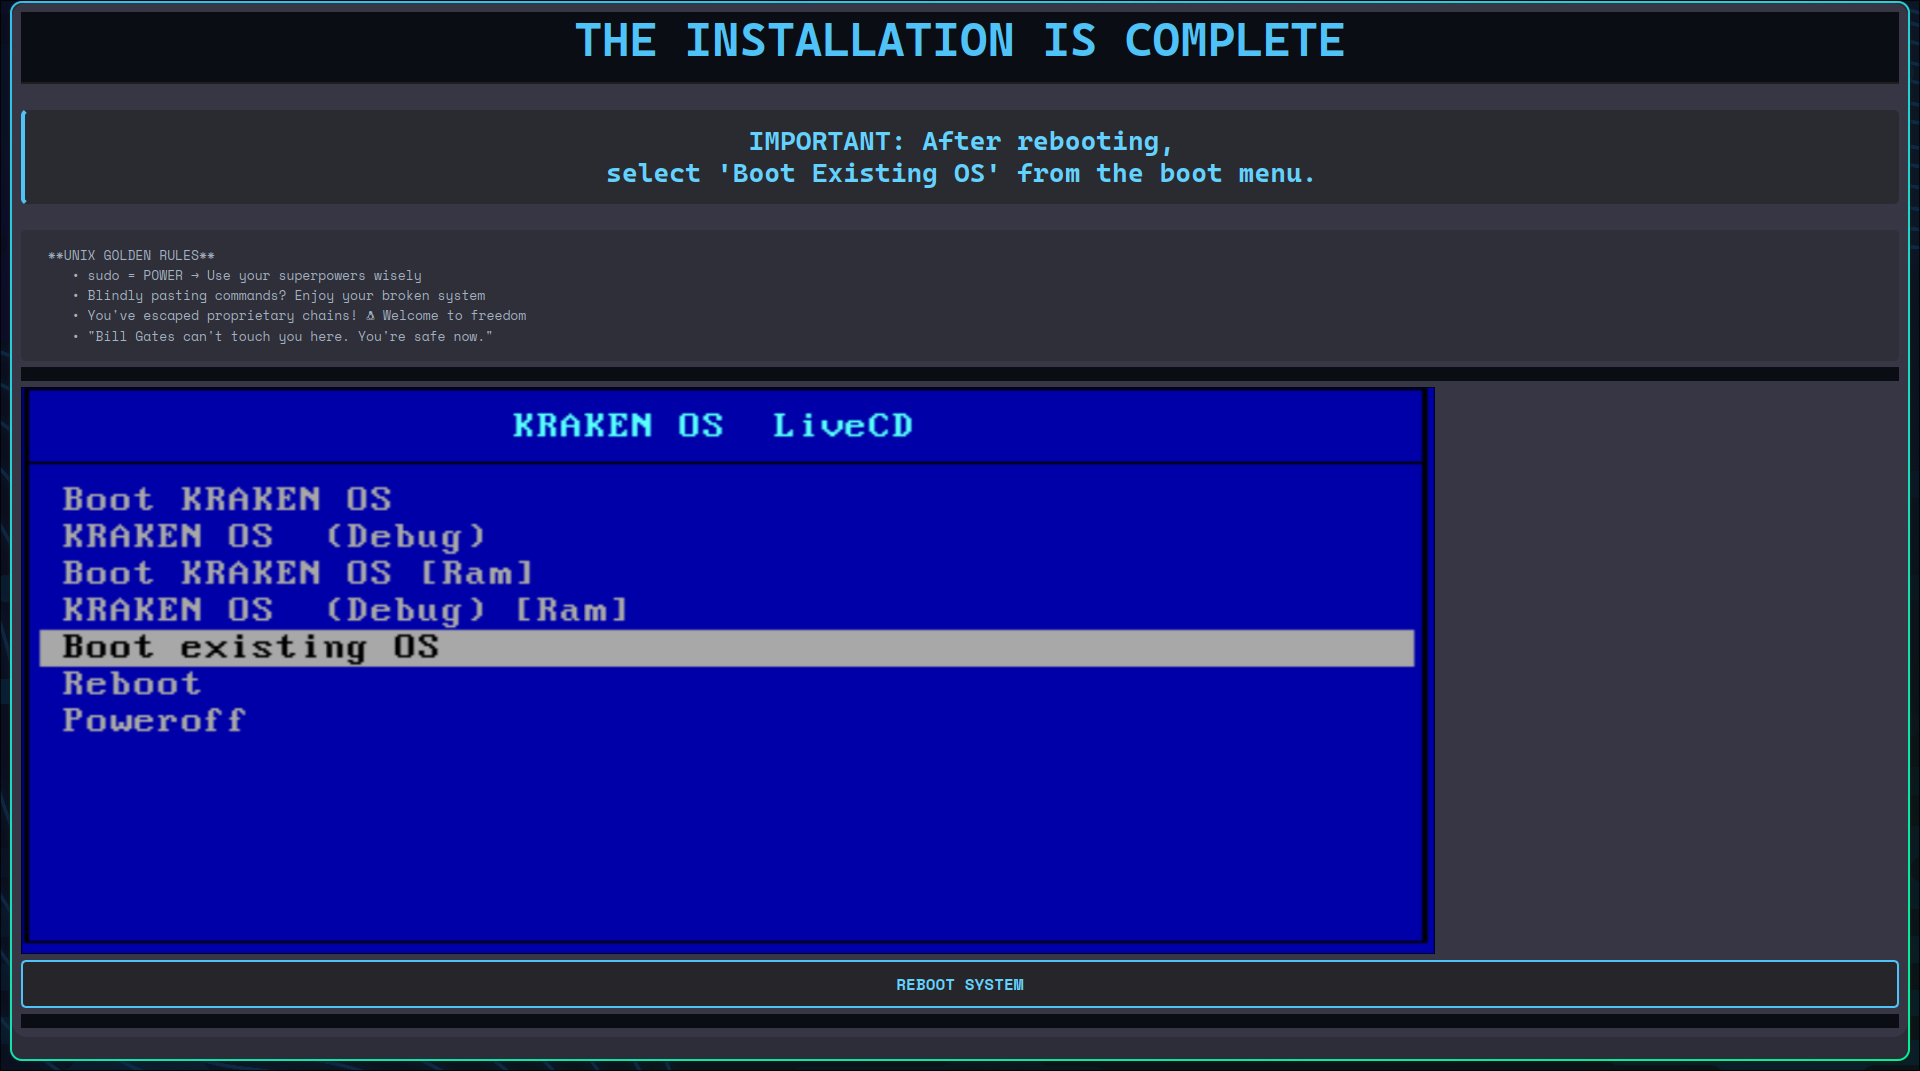
\includegraphics[width=1\textwidth, height=10cm]{images_pfe/finish.png}
  \caption{Interface de confirmation de redémarrage dans \textsc{Kraken Installer}}
  \label{fig:reboot-page}
\end{figure}
\label{subsec:reboot}

\textbf{Fonctionnalité finale} :
\begin{itemize}
    \item Bouton de confirmation (\texttt{QPushButton}) demandant à l'utilisateur :
    \begin{itemize}
        \item De valider le redémarrage du système
        
    \end{itemize}
 
 \end{itemize}




\textcolor{blue}{Le code source du  lapplication  graphique d’installation est disponible dans  \cite{installateur_gui}.}
\subsection{ISO}

Maintenant, après avoir préparé tous les composants, on peut générer l'image ISO.\


\medskip
\clearpage
\textbf{Exemple de structure d'un fichier ISO :}

\begin{figure}[H]
  \centering
  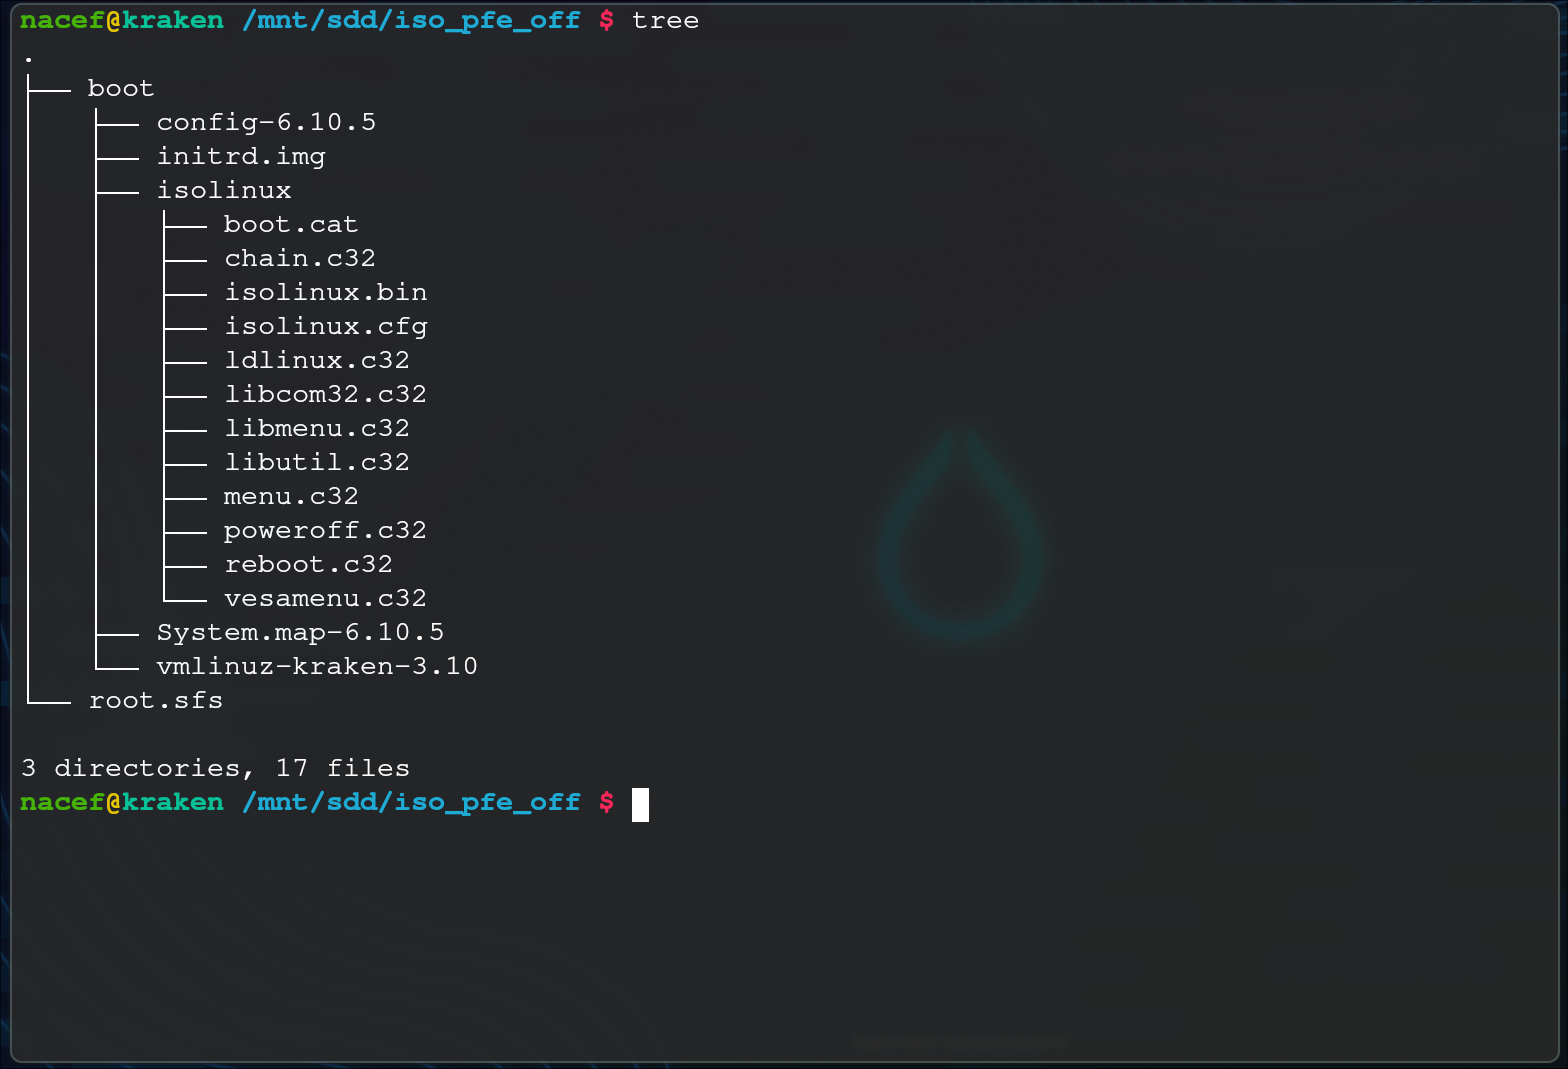
\includegraphics[width=1\textwidth, height=10cm]{images_pfe/isocontent.png}
  \caption{Contenu du fichier ISO avant sa génération}
  \label{fig:iso_directory_content}
\end{figure}

\medskip

\textbf{Explication :}\\
Comme le montre la figure, à la racine du répertoire, nous avons le fichier \texttt{squashfs} généré précédemment ainsi qu'un répertoire nommé \texttt{boot}.\\
Dans ce répertoire \texttt{boot}, on trouve les fichiers \texttt{initrd.img}, l’image du noyau, les fichiers \texttt{config} et \texttt{System.map}, ainsi qu’un dossier \texttt{isolinux} contenant notre chargeur d’amorçage (SYSLINUX).\\
Ce dossier \texttt{isolinux} contient des fichiers critiques comme \texttt{isolinux.cfg} \textcolor{blue}{(créé précédemment \ref{fig:isolinux})}, ainsi que plusieurs bibliothèques et modules d’amorçage tels que \texttt{poweroff.c32}, \texttt{reboot.c32}, \texttt{libutil.c32} et \texttt{libmenu.c32}.

\medskip
\bigbreak

\textbf{Exemple de commande pour générer une ISO amorçable :}

\textbf{Remarque :} les grandes distributions créent généralement leurs propres outils pour la génération d'images ISO.\\
Par exemple, la distribution Arch Linux utilise son propre outil appelé \texttt{archiso}, tandis que la distribution Red Hat utilise \texttt{lorax}.\\
Malheureusement, nous n'avons pas encore eu le temps de développer notre propre outil, mais nous envisageons de le faire bientôt.\\
À ce stade, nous utilisons des outils comme \texttt{xorriso} et \texttt{mkisofs} pour générer l'ISO.
\begin{verbatim}
sudo mkisofs \
  -V "KRAKEN-OS" \
  -o /home/nacef/krakenos-3.10.iso \
  -b boot/isolinux/isolinux.bin \
  -c boot/isolinux/boot.cat \
  -no-emul-boot \
  iso-pfe-off
\end{verbatim}

\textbf{Explication des options :}
\begin{itemize}
  \item \texttt{-V "KRAKEN-OS"} : définit l'étiquette de l'ISO
  \item \texttt{-o} : chemin de sortie du fichier ISO
  \item \texttt{-b} : image de démarrage de isolinux
  \item \texttt{-c} : fichier catalogue de démarrage de isolinux
  \item \texttt{-no-emul-boot} : requis pour rendre l’image amorçable
  \item \texttt{iso-pfe-off} : répertoire contenant la structure du système de fichiers ISO
\end{itemize}

\medskip

\textbf{Exemple : détection du type, de la taille et de l’intégrité de l’image ISO à l’aide des commandes \texttt{file}, \texttt{du}, et \texttt{md5sum} :}

\begin{figure}[H]
  \centering
  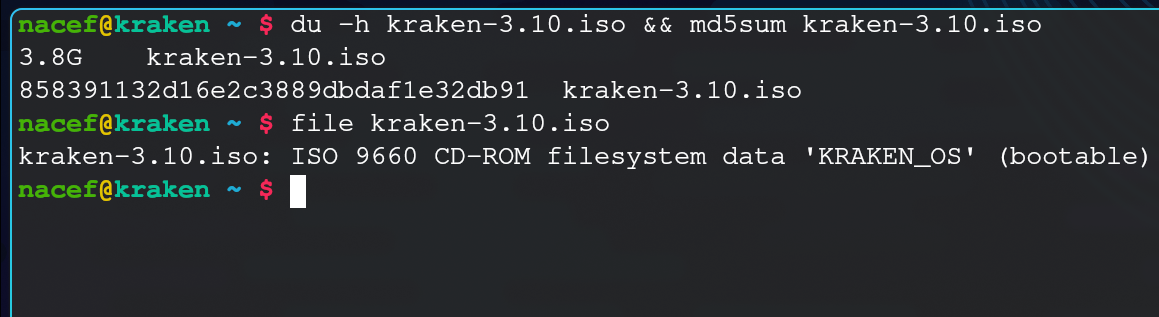
\includegraphics[width=1\textwidth, height=10cm]{images_pfe/fileisoofff.png}
  \caption{Type du fichier ISO, taille et vérification d'intégrité}
  \label{fig:iso_type}
\end{figure}

\medskip
\textbf{Résumé :}\\
Lorsque l'ISO est démarrée (ex: machine virtuelle), le BIOS/UEFI charge le bootloader ISOLINUX (dans \texttt{isolinux/}), lit le fichier \texttt{isolinux.cfg}, affiche le menu, puis charge le noyau et l'initrd spécifiés dans l'entrée sélectionnée.\\

\texttt{initrd.img} exécute alors le script \texttt{init} \textcolor{blue}{(créé précédemment \ref{fig:initscript})} via \texttt{busybox}. Ce script :\\
1. Monte les systèmes de fichiers virtuels (\texttt{/proc}, \texttt{/sys}, \texttt{/dev})\\
2. Détecte et monte le contenu de l'ISO\\
3. Monte le système SquashFS (\texttt{root.sfs})\\
4. Effectue un \texttt{chroot} dans ce système.\\

Le contrôle est alors transféré à \texttt{System V}, qui démarre l'environnement KDE Plasma et lance l'application graphique d'installation \textcolor{blue}{(section \ref{secc:graphapp})}, permettant d'installer le système sur disque.

\bigbreak
Le lien de téléchargement de l’image ISO est disponible ici : \cite{iso_link}.

Des étapes supplémentaires pour le téléchargement et un guide d’utilisation de notre distribution  sont  disponibles ici :\cite{guide_iso}.
